%
% HSR LaTex Template
% Copyright 2012, Florian Bentele / modified 2015 - Martin Stypinski
%
% Complete LaTex template for thesis at HSR, customized
% for Prof. Dr. Peter Heinzmann
%
%
% This document is free software: you can redistribute
% it and/or modify it under the terms of the GNU
% General Public License as published by the Free
% Software Foundation, either version 3 of the License,
% or (at your option) any later version.
%
% This document is distributed in the hope that it will
% be useful, but WITHOUT ANY WARRANTY; without even the
% implied warranty of MERCHANTABILITY or FITNESS FOR A
% PARTICULAR PURPOSE. See the GNU General Public
% License for more details.
%
% You should have received a copy of the GNU General
% Public License along with this document. If not, see
% <http://www.gnu.org/licenses/>.
%

\newcommand{\kiru}{Kirusanth Poopalasingam}
\newcommand{\styp}{Martin Stypinski}
\newcommand{\aeme}{Marcel Amsler}

% commands for tick and cross
\newcommand{\checkgood}{\ding{51}}
\newcommand{\checkbad}{\ding{55}}


\documentclass[11pt]{hsrthesis}

% The following snippet is copied from this stack overflow answer
% http://stackoverflow.com/a/3175141
% It sets the color right for lstlisting, so that we 
% can include code snippet
\definecolor{dkgreen}{rgb}{0,0.6,0}
\definecolor{gray}{rgb}{0.5,0.5,0.5}
\definecolor{mauve}{rgb}{0.58,0,0.82}

\lstset{frame=tb,
	language=Java,
	aboveskip=3mm,
	belowskip=3mm,
	showstringspaces=false,
	columns=flexible,
	basicstyle={\small\ttfamily},
	numbers=none,
	numberstyle=\tiny\color{gray},
	keywordstyle=\color{blue},
	commentstyle=\color{dkgreen},
	stringstyle=\color{mauve},
	breaklines=true,
	breakatwhitespace=true,
	tabsize=3
}

\makeindex

\makeglossaries
\newglossaryentry{Clusteranalyse}{
	name=Clusteranalyse,
	description={Ein Verfahren zur Feststellung von Ähnlichkeiten in Datenbeständen},
	first={Clusteranalyse}
}

\newglossaryentry{AMQP}{
	name=AMQP,
	description={Advanced Message Queuing Protocol, wird verwendet für die Übertragung der Messages an den Message Broker.}
}

\newglossaryentry{APK}{
	name=APK,
	description={ Android Package, ist das Datenformat indem Android Apps gespeichert werden. }
}

\newglossaryentry{OTG}{
	name=OTG,
	description={ USB On-the-go, ist der Standard um eine direkte Kommunikation zwischen USB-Geräten ohne Host-Controller zu ermöglichen. In unserem Fall um ein USB Gerät an ein Smartphone anzuschliessen. }
}

\newglossaryentry{MOM}{
    name=MOM,
    description={Message Oriented Middleware, ist Abstraktionsschicht zur Kommunikation zwischen Systemen}
}

\newglossaryentry{Message-Producer}{
	name=Message Producer,
	description={ Bei einem Messaging-System oder einer MOM (Message Oriented Middleware) gibt es immer Message Producer und Message Consumer. Ein Message Producer erstellt Nachrichten, ein Message Consumer hingegen empfängt und verarbeitet diese. }
}


\newglossaryentry{MAVLink}{
	name=MAVLink,
	description={ MAVLink ist ein reines Header-Protokoll, dass es ermöglicht unbemannte Fahr- und Flugzeuge zu kontrollieren. Es kann über verschiedene Protokolle laufen (USB, UDP, TCP) }
}

\newglossaryentry{Flight-Controller}{
	name=Flight-Controller,
	description={ Der Flight-Controller ist der Kern der Drohne, übernimmt die Stabilisierung und Steuerung der Rotoren. Wird über das MAVLink Protokoll mit Befehlen gesteuert. }
}

\newglossaryentry{CGAL}{
	name=CGAL,
	description={The Computational Geometry Algorithms Library ist eine C++ Bibliothek die einfachen und effizienten Zugang zu Algorithmen auf geometrischen Objekten ermöglicht. Sie bietet unter anderem folgende Algorithmen: ConvexHull, AlphaShape, MeshGeneration, ShapeAnalysis, uvm.}
}

\newglossaryentry{SFCGAL}{
	name=SFCGAL,
	description={Simple Feature CGAL ist eine Bibliothek die mit Geometrie Typen aus dem OGC Standart arbeitet. Es kann somit mit den bekannten Datentypen die im Open Source GIS Umfeld weit verbreitet sind, gearbeitet werden.}
}

\newglossaryentry{OGC}{
	name=OGC,
	description={Open Geospatial Consortium ist eine Organisation die viele GIS relevante Standarts im Open Source Bereich geschaffen hat.}
}

\newglossaryentry{MIT-Lizenz}{
	name=MIT-Lizenz,
	description={Eine Software-Lizenz, die es jedem erlaubt den Code in jeder Art weiterzuverwenden.}
}

\newglossaryentry{BEC}{
	name=BEC,
	description={Battery Eliminator Circuit ist eine im RC-Modellbau verwendete Terminologie für eine Spannungsstabilisierungsschaltung, um konstante Spannung zu gewährleisten.}
}

\newglossaryentry{JTS}{
	name=JTS,
	description={Java Topology Suite ist ein API für 2D Objekte und deren Operationen. Sie erfüllt den Open Geospatial Consortium Standard und implementiert somit die gleichen Objekte wie PostGIS.}
}

\newglossaryentry{UAV}{
	name=Unpiloted Aerial Vehicle (UAV),
	description={Flugzeug welches Autonom fliegen kann, beispielsweise eine Drohne.}
}

\newglossaryentry{CRUD}{
	name= CRUD,
	description={Abkürzung für C = Create, R = Read, U = Update, D = Delete. Es wird zur Bezeichnung von Operationen auf einem Model/Resource verwendet. Beispielsweise sollen Benutzer erstellt (Create), angesehen (Read), geändert (Update) und gelöscht (Delete) werden können.}
}

\newglossaryentry{DTO}{
	name= Data Transfer Object (DTO),
	description={Objekte die übertragen werden können und keine Abhängigkeiten zum System haben.}
}

\newglossaryentry{E2E-Test}{
	name= E2E-Test,
	description={Diese Art von automatisierten Test simuliert einen Benutzer. Typischerweise wird die zu testende Applikation in einem Browser geöffnet und automatisiert die gewünschten Aktionen mit Klicks ausgeführt.}
}

\newglossaryentry{Integration-Test}{
	name= Integration-Test,
	description={Integration-Tests testen normalerweise ein ganzes System ohne Benutzeroberfläche aber mit Datenbank und anderen Abhängigkeiten.}
}

\newglossaryentry{Unit-Tests}{
	name= Unit-Tests,
	description={Automatisierte Tests, die nur eine Methode testen, ohne irgendwelche Abhängigkeiten.}
}

\newglossaryentry{Single-Page-Applications}{
	name= Single-Page-Applications,
	description={Eine Webseite, die dynamisch verändert wird, ohne dass der Server ihr neuen HTML-Code schicken muss.}
}


\newglossaryentry{JMS}{
	name=JMS,
	description={Java Messaging Service. API um aus Java einen Message Broker anzusprechen.}
}

\newglossaryentry{DBMS}{
	name=DBMS,
	description={Ein Database Management System dient zur Verwaltung und zur Abfrage einer Datenbank. Bekannte Systeme sind Oracle, MSSQL und PostgreSQL}
}




\begin{document}
\newcommand{\thesistitle}{Project Helin}
\newcommand{\thesissubtitle}{Drone delivery as a service}
\newcommand{\thesisauthora}{Marcel Amsler}
\newcommand{\thesisauthorb}{Kirusanth Poopalasingam}
\newcommand{\thesisauthorc}{Martin Stypinski}
\newcommand{\professor}{Prof. Dr. Markus Stolze}
\newcommand{\thesistype}{Bachelorarbeit}
\newcommand{\departement}{Abteilung Informatik}
\newcommand{\school}{Hochschule für Technik Rapperswil}
\newcommand{\term}{Frühlingssemester 2016}
\newcommand{\thedate}{\today}
\newcommand{\timeperiode}{22.02.2015 - 17.06.2015}
\newcommand{\workload}{360 Stunden, 12 ECTS pro Student}
\newcommand{\linktothesis}{https://github.com/Project-Helin/}

\maketitle


\newpage

\pagenumbering{roman}


% The main content
%%%%%%%%%%%%%%%%%%


\cleardoublepage
\phantomsection
\addcontentsline{toc}{chapter}{Eigenständigkeitserklärung}
\chapter*{Eigenständigkeitserklärung}

%\chapter{Eigenständigkeitserklärung}
Wir erklären hiermit,
\begin{itemize}
	\item{dass wir die vorliegende Arbeit selber und ohne fremde Hilfe durchgeführt haben, ausser
derjenigen, welche explizit in der Aufgabenstellung erwähnt sind oder mit dem Betreuer
schriftlich vereinbart wurden,}
	\item{dass wir sämtliche verwendeten Quellen erwähnt und gemäss gängigen wissenschaftlichen
Zitierregeln korrekt angegeben haben,}
	\item{dass wir keine durch Copyright geschätzten Materialien (z. B. Bilder) in dieser Arbeit in
unerlaubter Weise genutzt haben.}
\end{itemize}
\begin{verbatim}




\end{verbatim}
Rapperswil, den \today
\begin{verbatim}







\end{verbatim}
\centering
\includegraphics[width=1.0\paperwidth]{unterschriften/alle.jpg}
\begin{tabular*}{\textwidth}{p{0cm}>{\centering\arraybackslash}m{4.8cm}>{\centering\arraybackslash}m{4.8cm}>{\centering\arraybackslash}m{4.8cm}p{0cm}}
	& Marcel Amsler & Kirusanth Poopalasingam & Martin Stypinski & \\
\end{tabular*}

\newpage
\addcontentsline{toc}{chapter}{Danksagung}
\chapter*{Danksagung}
Zunächst möchten wir uns an dieser Stelle bei all denjenigen bedanken, die uns während der Anfertigung dieser Arbeit unterstützt und motiviert haben.
\begin{itemize}
	\item{}
\end{itemize}
\newpage
\addcontentsline{toc}{chapter}{Abstract}
\chapter*{Abstract}
YOLO Abstract 1
\newpage
\cleardoublepage
\phantomsection
\addcontentsline{toc}{chapter}{Management Summary}
\chapter*{Management Summary}
\section*{Ausgangslage}
Drohnen, die autonom fliegen und nicht mehr gesteuert werden müssen, gehört die Zukunft. Sie werden sicherer sein als heutige, von Menschen gesteuerte Drohnen und erlauben ein grösseres Einsatzgebiet. Firmen wie Amazon und die schweizerische Post planen bereits heute den Einsatz von Drohnen zur automatischen Auslieferung von Paketen. Doch vielen Anbietern bleibt diese Möglichkeit verwehrt, obwohl auf dem Markt eine Vielzahl von Komponenten zur Verfügung steht, um autonome Drohnen selbst zu bauen und zu betreiben. Die bestehenden Lösungen steuern aber immer nur eine Drohne gleichzeitig über Funk und bieten nur eine begrenzte Reichweite. Ausserdem existiert noch keine frei verfügbare Software, um automatisierte Dienstleistungen mit Drohnen anzubieten oder eine autonome Flotte zu verwalten.

\section*{Vorgehen / Technologien}
Um zu zeigen, was mit heutigen Technologien und Standardkomponenten bereits möglich ist, wurde ein Demonstrationssystem mit zwei selbst gebauten Drohnen entwickelt. \\

Ein Smartphone, welches auf der Drohne montiert ist, ermöglicht die Kommunikation mit der Plattform, aber auch eine Benutzerinteraktion über das Display. Bei einer eingehenden Bestellung von der Bestell-App wird automatisch eine Route zum Kunden berechnet und einer verfügbaren Drohne zugewiesen. Sobald diese beladen ist, fliegt sie autonom zum Kunden, liefert das Produkt aus und kehrt wieder zurück. Dabei bleibt die Drohne in den vordefinierten, sicheren Flugzonen und weicht somit statischen Hindernissen aus. Eine Fernsteuerung wird nicht mehr benötigt, das System ist komplett autonom. Die App dient als Schnittstelle zwischen der cloudbasierten Verwaltungssoftware und der Drohnensteuerung, welche bereits grundsätzliche Funktionen wie GPS, automatische Stabilisierung und sogar einen programmierbaren Autopiloten bietet.

\section*{Ergebnisse}
Das System zeigt erst einen Bruchteil der Möglichkeiten, die in Zukunft von autonomen Drohnen übernommen werden können. Beispielsweise können Videoaufnahmen, Infrastrukturüberwachung oder Katastrophenhilfe als Angebote integriert werden. \\

Wir sind überzeugt davon, dass die entwickelte Plattform als Denkanstoss für diese Branche und die Politik dienen kann, um die Technologien und Gesetzeslagen soweit zu verbessern, dass Dienstleistungen von Drohnen bald überall zur Verfügung stehen werden.

\newpage
\addcontentsline{toc}{chapter}{Aufgabenstellung}
\chapter*{Aufgabenstellung}
\label{cha:aufgabenstellung}

\section*{Betreuer \& Auftraggeber}
\begin{itemize}
	\item{\textbf{Betreuer:} Prof Dr. Markus Stolze, Dozent für Informatik HSR}
	\item{\textbf{Co-Referent:} Prof Beat Stettler, Dozent für Informatik HSR}
	\item{\textbf{Experte:} TBD}
	\item{\textbf{Anwendungspartner:} Abteilung Informatik HSR}		
\end{itemize}

\section*{Ausgangslage}
Multicopter haben in den letzten Jahren grosse technologische Fortschritte erlebt. Sie sind leichter, einfacher zu bedienen, leistungsfähiger und preiswerter geworden, so dass sie auch für kleine Geschäfte und Privatpersonen erschwinglich geworden sind. 
Ein möglicher Anwendungsbereich von Multicoptern ist die schnelle Auslieferung von Produkten. So ist es im Prinzip schon heute möglich mit einem Multicopter einen Defibrillator punktgenau zu einer bedürftigen Person an einem Open-Air-Konzert zu bringen. Allerdings erlaubt die aktuelle Gesetzgebung keine automatisch gesteuerten Flüge von Multicoptern. Zudem ist auch manuell gesteuerte Flüge „auf Sicht“ in der Nähe von grösseren Menschenansammlungen nicht erlaubt. Da die Gesetzliche Lage aktuell im Fluss ist, kann es sein dass diese Limitationen schon bald nicht mehr gelten und es somit interessant wäre eine Software-Platform zu erstellen mit der automatisch gesteuerte Zustellung von Produkten mit Multicoptern abgewickelt werden können.  

\section*{Ziele der Arbeit}
In dieser Arbeit sollen Komponenten eine erweiterbare open-source Software-Plattform mit den folgenden vier Komponenten erstellt werden 
\begin{enumerate}
	\item{Ein Prototyp einer Android App mit der Produkt-Bestellungen beim System abgegeben werden können. Die Android App soll den Standort des Bestellers mittels GPS bestimmen und zusammen mit der Produktwahl an die zentrale Management Anwendung übertragen. Diese App soll bewusst einfach gehalten sein und soll Themen wie Bezahlung ausser Acht lassen.}
	\item{Eine prototypische Konfigurationsanwendung mit der sich Multicopter, Multicopter-Startplätze, Flugkorridore und Produktlisten erstellen und verwalten lassen.}
	\item{Eine gut getestete, wartbare und optimierte Management Anwendung welche Aufträge der Bestell-App entgegennimmt, automatisch einen freien Multicopter für die Durchführung der Zulieferung bestimmt, den Auftrag an die Multicopter-App übermittelt und die Durchführung des Auftrags überwacht. Dabei soll auch das Abbrechen eines Auftrags mitten im Flug möglich sein.}
	\item{Eine gut getestete und wartbare Multicopter App die für ein Android-Phone welches auf dem Multicopter montiert ist optimiert ist. Die Android App ist über das Handy-Netz in steter Kommunikation mit der Management Anwendung. Die App meldet die Position des Multicopters in regelmässigen Abständen und ist in der Lage im Flug Befehle der Management Anwendung an den Steuerungs-Controller auf dem Multicopter über eine für Multicopter standardisierte Schnittstelle zu übertragen.}
\end{enumerate}
Die Aufgabe umfasst neben der Erstellung der oben genannten Software-Komponenten auch die Zusammenstellung der Bestellliste für den Aufbau eines Demonstrators mit zwei flugfähigen Drohnen, sowie die Demonstration eines realistischen Bestell- und Auslieferungsszenarios. Hierzu sind zum Beispiel Lösungsvorschläge für die für Besteller gefahrlose Ablieferung zu erarbeiten. Neben der Software und der Multicopter-Hardware ist ein wichtiges Produkt dieser Arbeit eine Video-Dokumentation die zeigt inwieweit sich mit den erstellten Software und Hardwarekompoenten ein realistischen Bestell- und Auslieferungsszenarios realisieren liess.
\section*{Dokumentation}
Über diese Arbeit ist eine Dokumentation gemäss den Richtlinien der Abteilung Informatik zu verfassen. Die Dokumentation ist vollständig auf CD/DVD in einem Exemplar abzugeben (Exemplar für das Sekretariat Informatik), sowie ein Download-Link für Prof. Stolze und weitere Exemplare nach Absprache mit dem Co-Referenten (B. Stettler) und dem Experten (@@@@@).
\\
Zudem ist eine kurze Projektresultatdokumentation im öffentlichen Wiki von Prof. M. Stolze zu erstellen.
\section*{Weitere Regeln und Termine }
Im Weiteren gelten die allgemeinen Regeln zu Bachelor und Studienarbeiten \\
"Abläufe und Regelungen Studien- und Bachelorarbeiten im Studiengang Informatik" (HSR Intranet)\\ \url{https://www.hsr.ch/Ablaeufe-und-Regelungen-Studie.7479.0.html}\\
Der Terminplan ist hier ersichtlich (HSR Intranet)
\\
\url{https://www.hsr.ch/Termine-Bachelor-und-Studiena.5142.0.html}
\section*{Rechte}
Die resultierende Software und Dokumentation soll als open-source Software (MIT Lizenz) publiziert werden. Die Multicopter Hardware wird von der HSR beschafft und bleibt Eigentum der HSR. Es wird durch alle Parteien sicher gestellt, im Source-Code und im Impressum der Anwendung die originale Urheberschaft durch die HSR Studenten weiterhin sichtbar bleibt.
\\
Der Bericht der Bachelorarbeit (ohne geheime Anhänge) wird von der HSR im E-Prints Respository der HSR (eprints.hsr.ch) elektronisch veröffentlich. Titel und Abstract der Arbeit dürfen von der HSR und den Studierenden schon während der Arbeit kommuniziert werden.
\section*{Beurteilung}
Eine erfolgreiche Bachelorarbeit zählt 12 ECTS-Punkte pro Studierenden. Für 1 ECTS Punkt ist eine Arbeitsleistung von ca. 25 bis 30 Stunden budgetiert. Entsprechend sollten ca. 350h Arbeit für die Bachelorarbeit aufgewendet werden. Dies entspricht ungefähr 25h pro Woche (auf 14 Wochen) und damit ca. 3 Tage Arbeit pro Woche pro Student.
Für die Beurteilung ist der HSR-Betreuer verantwortlich. Die Bewertung der Arbeit erfolgt entsprechend der verteilten Kriterienliste.
Die Aufgabenstellung wurde am @@@@@@ vorbesprochen. Die definitive Aufgabenstellung wurde am @@@@ beschlossen. 
\begin{verbatim}


\end{verbatim}
Rapperswil, @@@@@@@ Prof. Dr. Markus Stolze \\
Institut für Software, Hochschule für Technik Rapperswil

% Table of content
% % % % % % % % %
\newpage
\addcontentsline{toc}{chapter}{Inhaltsverzeichnis}
\tableofcontents
\newpage

\pagenumbering{arabic}
\setcounter{page}{1}



\part{Technischer Bericht}
\chapter{Einleitung und Übersicht}

\section{Einleitung}

Ziel dieser Arbeit ist es eine Multi-Tenant-fähige Plattform zu konzipieren, zu entwickeln und zu veröffentlichen. Diese soll es Anbietern von Produkten und Services ermöglichen, ihre Drohnen für einen begrenzten Zeitraum oder für bestimmte Aufgaben zur Verfügung zu stellen. Das ausführen einer Aufgabe soll, bis auf das beladen der Drohne, komplett automatisiert ablaufen. \\

Sobald ein Kunde eine Bestellung über eine App tätigt, wird automatisch eine Route zu seiner Position berechnet, die über vordefinierte, sichere Zonen führt. Über ein auf der Drohne angebrachtes Smartphone erhält der Drone-Operator dann Anweisungen für die Beladung. Sobald die Vorbereitungen abgeschlossen sind, bewegt sich die Drohne dann mit Hilfe von GPS entlang der berechneten Route, erfüllt ihre Aufgabe und kehrt wieder zurück. Während der Mission werden laufen Telemetriedaten an den Server geschickt, welcher diese für den Anbieter visualisiert.\\

Project Helin wird als Open-Source Software veröffentlicht und kann dann von einem oder mehreren Anbietern gehostet und weiterentwickelt werden.\\

In der weiteren Dokumentation werden die Anforderungen, die Architektur, die wichtigsten Punkte der Umsetzung sowie der Aufbau eines Anwendungsbeispiels mit zwei echten Drohnen beschrieben.

\section{Ausgangslage}

Alle Multicopter verfügen bereits in der Grundausstattung über einen \Gls{Flight-Controller}, der die Befehle der Fernbedienung in Steuerbefehle für die Motoren übersetzt. Zusätzlich nutzen viele Modelle zusätzliche Sensoren (GPS, Beschleunigungsmesser) um autonome Flüge zu ermöglichen und den Copter stabil halten. \\

Um laufend Telemetriedaten zu erhalten und Funktionen steuern zu können, wird in den meisten Fällen über Funk mit dem Copter kommuniziert. Dafür wird ein Mobiles Gerät verwendet (Smartphone, Tablet, Notebook) auf dem eine Bodensationssoftware läuft (z.B. Tower-App, Missionplaner, oder DJI Go App). Dies ermöglicht die Steuerung in einem Umkreis von ca. 2km.  \\

Zusätzlich können mit Hilfe einer Bodenstationssoftware fixe Routen auf den Flight-Controller gespeichert werden, die dann im Automatikmodus autonom geflogen werden.\\

Dieses bewährte System hat allerdings einige Einschränkungen: 

\begin{itemize}
	\item{Reichweite ist begrenzt}
	\item{Daten der Flüge sind nur für einen Benutzer einsehbar (Lokale Speicherung der Daten)}
	\item{Flugrouten müssen von Hand eingegeben werden}
	\item{Keine zentrale Komponente, auf die andere Systeme (z.B. Bestellapps) zugreifen und Aktionen der Drohnen auslösen können.}
\end{itemize}

Project Helin soll nun alle diese Einschränkungen aufheben. Damit können Anbieter neue Dienstleistungen erbringen, die nur mit autonomen Flugdrohnen in einer sinvollen Geschwindigkeit und Qualität möglich sind.

Bis jetzt gibt es kein vergleichbares System, dass mit Drohnen über das Internet live kommuniziert und gleichzeitig die Anbindung von zusätzlichen Systemen erlaubt.

\section{Gesetzliche Rahmenbedingungen}

Für den Flug mit Drohnen in der Schweiz gelten die Vorgaben des Bundesamt für Zivilluftfahrt BAZL.
Drohnen dürfen ohne Bewilligung geflogen werden, solange das Gesamtgewicht von 30kg nicht überschritten wird \cite{drohne-bazl}.
Auch für den Betrieb über Menschenansammlungen bzw. im Umkreis von 100 Metern ist eine Bewilligung erforderlich.
Ein autonomer Flug ist gestattet, solange der Pilot die Drohne in Sichtweite hat und manuell eingreifen kann.
\\

In anderen Ländern gelten ähnliche Bedingungen, so ist etwa in den Staaten eine Registration für Freizeitdrohnen von 250g bis 25kg erforderlich \cite[Seite 26]{pwc-drone}.
In vielen Ländern werden die Gesetzlichen Rahmenbedingungen angepasst, so dass auch Drohnen ausser Sichtweite betrieben werden können.
Zum Beispiel kann in Polen eine Lizenz, nach theoretischer und praktischer Prüfung, erworben werden um Flüge ausser Sichtweite durchzuführen \cite[Seite 21]{pwc-drone}.

Wir hoffen, dass die Gesetzte dahingehend angepasst werden, um einen kommerziellen Einsatz von autonomen Drohnen zu begünstigen. 

\section{System Kontext}

Project Helin hat drei verschiedene Nutzerarten: Customers (Kunden), Administrators(Anbieter) und Drone-Operators. Diese werden im Kapitel Anforderung noch genauer beschrieben.\\

In Abbildung \ref{fig:system-context-diagram} sind die externen Schnittstellen, sowie die Aktoren dargestellt. Google OAuth und Paypal werden auf der Customer-App für die Authentifizierung und das Payment eingesetzt. Die 3DR-Service-App wird auf dem Onboard App benötigt um die Kommunikation mit dem Flight-Controller der Drohne zu ermöglichen. Für die Kartendarstellungen auf der Administrations Webseite werden von Open Street Map gehostete Karten verwendet.


\begin{figure}[h]
\includegraphics[width=1.0\textwidth]{images/system-context-diagram.png}
\caption{System Kontext Diagram mit externen Schnittstellen }
\label{fig:system-context-diagram}
\end{figure}










\chapter{Anforderungen}

\section{Benutzer und Personas}


Die Benutzer der Project Helin Plattform teilen sich in zwei Gruppen auf, welche in dieser Arbeit berücksichtigt werden.

\subsection{Service-Nutzer}

Service-Nutzer verwenden nur die Service App um einen Service oder ein Gut an ihre Position zu bestellen.

\subsubsection{Persona Diego}

\begin{figure}[h]
\includegraphics[width=.35\textwidth]{images/persona-diego.jpg}
\caption{Persona Diego: Freie Lizenz; Quelle }
	%\url{http://blog.placeit.net/free-avatar-pack/}}
\label{fig:diego}
\end{figure}

Er ist \textbf{23 Jahre alt} wohnt in einer WG in Uster.\\

Diego hat eine Informatik-Lehre mit BMS abgeschlossen und ist auf der Suche nach einer neuen beruflichen oder schulischen Herausforderung.

\paragraph{Technisches Verhalten}

Arbeitet täglich acht Stunden mit dem PC. Nutzt gerne neue Technologien. Besitzt ein Android-Smartphone der neusten Generation. Die Android Updates macht er immer sofort. Interessiert sich für neue Technologien und sieht sich regelmässig Kickstarter Projekte an.\\

\paragraph{Ziele}

Möchte sich weiterbilden und neue Herausforderungen finden. Möchte neue Technologien entdecken und einsetzen.\\

\subsection{Administratoren}

Administratoren verwenden die Project Helin Plattform um eine Flotte von Drohnen zu verwalten. Sie nutzen dazu die Webseite der Plattform und kümmern sich um das definieren von Flugzonen, Services und Gütern.

\subsubsection{Persona Stefanie}
\begin{figure}[h]
	\includegraphics[width=.35\textwidth]{images/persona-stefanie.jpg}
	\caption{Persona Stefanie: Freie Lizenz; Quelle} %\url{http://blog.placeit.net/free-avatar-pack/}}
	\label{fig:stefanie}
\end{figure}


Carmen ist \textbf{35 Jahre alt} und lebt alleine in Zürich.

Sie unternimmt viel mit Freunden und reist gerne. Sie ist auf dem Land aufgewachsen und wohnt jetzt in Zürich.

Carmen arbeitet bei einer Eventagentur und hat eine Ausbildung als Eventmanagerin abgeschlossen.

\paragraph{Technisches Verhalten}
Sie nutzt den PC täglich bei der Arbeit, vor allem Planungstools und das E-Mail-Programm. Ausserdem ist sie zu Recherchezwecken viel im Internet unterwegs. Sie nutzt Chrome als Browser im Geschäft. Sie besitzt ein Samsung Galaxy S4, dass sie schon seit einigen Jahren verwendet. Zuhause hat sie keinen PC.

\paragraph{Kommunikationsverhalten}
Sie kommuniziert geschäftlich hauptsächlich per E-Mail. Mit Freunden kommuniziert sie über WhattsApp.

\paragraph{Ziele}
Sie möchte mit neuen und innovativen Ideen Events für Besucher spannender gestalten.

\section{Funktionale Anforderungen}

Die funktionalen Anforderungen leiten sich aus der Aufgabenstellung, sowie den mit dem Betreuer diskutierten Ideen ab.

\subsection{Administrator}
\begin{itemize}
\item Als Administrator möchte ich auf der Webseite einen Account erstellen können.
\item Als Administrator möchte ich ein Projekt erfassen können.
\item Als Administrator möchte ich auf eine Drohne dem Projekt hinzufügen können.
\item Als Administrator möchte ich alle Drohnen verwalten können (RUD).
\item Als Administrator möchte ich Güter verwalten können(CRUD).
\item Als Administrator möchte ich Services verwalten können (CRUD) (optional).
\item Als Administrator möchte ich Flug-, Lade- und Abwurfzonen verwalten können.
\item Als Administrator möchte ich Bestellungen verwalten können(CRUD).
\item Als Administrator möchte ich Missionen vor, nach, und während der Ausführung ansehen können.
\item Als Administrator möchte ich Missionen abbrechen können.
\end{itemize}

\subsection{Kunde}
\begin{itemize}
\item Als Service-Nutzer möchte ich eine App aus dem Google Play Store herunterladen können.
\item Als Service-Nutzer möchte ich die App nutzen ohne mich anzumelden zu müssen.
\item Als Service-Nutzer möchte ich in der App, aus einer Auswahl von Gütern und Services, eine Auswahl treffen können.
\item Als Service-Nutzer möchte ich eine Bestellung tätigen können.
\item Als Service-Nutzer möchte ich auf der Karte des Smartphones die Bewegung der Drohne verfolgen können.
\item Als Service-Nutzer möchte ich textuelle Updates über den Status meiner Bestellung erhalten.
\item Als Service-Nutzer möchte ich eine Bestellung stornieren können.
\end{itemize}

\subsection{Drone-Operator}
\begin{itemize}
	\item Als Drone-Operator möchte ich eine Android App mit Hilfe der heruntergeladenen APK installieren können.
	\item Als Drone-Operator möchte ich das Gerät bzw. die Drohne beim Server registrieren können.
	\item Als Drone-Operator möchte ich das Gerät bzw. die Drohne zu einer Organisation hinzufügen können.
	\item Als Drone-Operator möchte ich das OTG-Fähige Smartphone an einen MAV-Link kompatiblen Flight-Controller über USB anschliessen können.
	\item Als Drone-Operator möchte ich eine Verbindung zwischen App und Server über das Internet herstellen könnnen.
	\item Als Drone-Operator möchte ich eine Verbindung zwischen App und Flight-Controller herstellen können.
	\item Als Drone-Operator möchte ich den aktuellen Zustand der Verbindungen zur Drohne und zum Server sehen.
	\item Als Drone-Operator mpchte ich den aktuellen Status des Flight-Controllers, beispielsweise GPS und Batteriespannung sehen.
	\item Als Drone-Operator sehe wenn der Drohne eine neue Mission zugeteilt wurde.
	\item Als Drone-Operator möchte ich eine Liste von Gütern anzeigen lassen, die für die aktuelle Mission geladen werden müssen.
	\item Als Drone-Operator möchte ich eine Mission annehmen oder ablehnen können.
	\item Als Drone-Operator möchte ich die Beladung einer Drohne bestätigen können.
	\item Als Drone-Operator erhalte ich ein visuelles und akustisches Countdown-Signal bevor die Drohne startet.
	\item Als Drone-Operator möchte ich den Start der Drohne während des Countdowns verhindern können.
\end{itemize}


\section{Nichtfunktionale Anforderungen}

\subsection{Verbindungsabbruch}

\begin{tabular}{|p{.25\textwidth}|p{.75\textwidth}|} \hline
	Synopsis & Verbindungsabbruch der Onboard App zum Server soll keine negativen Auswirkungen auf die Mission haben.  \\ \hline
		
	Messbarkeit & Nach dem Start der Mission muss die Drohne auch ohne Verbindung zum Server die Mission abschliessen können. \\ \hline
\end{tabular}

\subsection{Sicherheit im Mittelpunkt}
\begin{tabular}{|p{.25\textwidth}|p{.75\textwidth}|} \hline
	Synopsis & Eine Drohne führt vor dem Freigeben der Motoren (Arming) einen Check durch, der prüft ob alle nötigen Voraussetzungen für einen Start erfüllt sind. Ausserdem müssen vor einem Start ebenfalls Voraussetzungen der Mission erfüllt sein, beispielsweise muss der Drone-Operator den Start freigeben. Sollte eine dieser Vorraussetzungen nicht erfüllt sein, darf die Drohne nicht starten.  \\ \hline
	
	Messbarkeit & Drohne darf nicht starten, falls der Pre-Flight-Check des Autopiloten nicht erfolgreich war oder Voraussetzungen für die aktuelle Mission nicht erfüllt sind. \\ \hline
\end{tabular}

\subsection{Verbindungswiederherstellung}
\begin{tabular}{|p{.25\textwidth}|p{.75\textwidth}|} \hline
	Synopsis & Nach einem Verbindungsabbruch zwischen dem Server und der Onboard App soll die Verbindung wiederhergestellt werden sobald wieder Internet verfügbar ist. \\ \hline
	
	Messbarkeit & Die Verbindung zwischen Server und App wird nach dem deaktivieren und wieder aktivieren der Internetverbindung innert 30 Sekunden wiederhergestellt.\\ \hline
\end{tabular}


\subsection{Nutzlast der Drohne}
\begin{tabular}{|p{.25\textwidth}|p{.75\textwidth}|} \hline
	Synopsis & Eine 1/2 Liter PET Flasche soll innerhalb von einem 500m Radius geliefert werden können. \\ \hline
	Messbarkeit & Im App kann ein Produkt mit einem Gewicht von 500g bestellt, und geliefert werden. \\ \hline
\end{tabular}


\section{Domain-Model}

Aus den Funktionalen Anforderungen ergibt sich das folgende Domainmodel.

\begin{figure}[h]
	\includegraphics[width=1.0\textwidth]{images/domainmodell.png}
	\caption{Domain-Model}
	\label{fig:domain-model}
\end{figure}


\chapter{Architektur}

\section{Ziele}

Die folgende Architektur soll es ermöglichen, eine Flotte von Drohnen automatisiert und zentralisiert zu verwalten. Die Kommunikation zwischen Server und Drohne muss ausserdem von beiden Seiten initiierbar sein (Push-Messages). Zusätzlich muss eine Schnittstelle für Kunden existieren, damit Bestellungen getätigt werden können. 


\section{Einschränkungen}

Da der Flight-Controller bereits vor Anfang der Arbeit bestellt wurde, wird dieser als vorgegebene Limitierung angesehen. Somit steht auch die Wahl auf MAVLink, für die Kommunikation mit der Drohne fest.  


\section{Übersicht}

Die Abbildung \ref{fig:architecture-overview} zeigt eine Übersicht der verschiedenen Tiers und Server-Komponenten.

\begin{figure}[H]
	\centering
	\includegraphics[width=0.8\textwidth]{images/Overview-Diagram.png}
	\caption{Übersicht der Project Helin Architektur }
	\label{fig:architecture-overview}
\end{figure}

\section{Logische Architektur}

\subsection{Komponenten Übersicht}

Abbildung \ref{fig:logical-architecture-overview} zeigt die Hauptkomponenten, sowie eine Übersicht der enthaltenen Layer und Packages. Ausserdem sind die Abhängigkeiten zu den wichtigsten externen Komponenten dargestellt. Hervorzuheben ist ebenfalls die gemeinsame Verwendung der Commons-Komponente. 

\begin{figure}[H]
	\includegraphics[width=1.0\textwidth]{images/logical-architecture-overview.png}
	\caption{Vereinfachte Übersicht der logischen Architektur und deren Komponenten }
	\label{fig:logical-architecture-overview}
\end{figure}

\section{Server-Komponente}

\subsection{Anforderungen}
Aus den in den Anforderungen definierten Zielen, ergeben sich für die Server-Komponente folgende Anforderungen:

\begin{itemize}
	\item Bietet Benutzeroberfläche für Administratoren
	\item Verwaltet CRUD für alle nötigen Klassen (siehe Domain Model)
	\item Verwaltet Verbindungen zu Onboard-Apps und Customer-Apps
	\item Berechnet Flugrouten basierend auf den erhaltenen Bestellungs-Koordinaten
\end{itemize}

\subsection{Layers}
Die Architektur des Servers basiert auf dem {MVC Pattern \cite{MVC}}, da dieses für CRUD Applikationen mit Benutzeroberfläche besonders geeignet ist und dafür viele geeignete Frameworks zur Verfügung stehen.\\

Für Komponenten die aus unterschiedlichen Controllern verwendet werden, wurde zusätzlich eine Service Komponente verwendet. Die Services stellen Abstraktionen für wichtige Funktionen wie das Messaging und die Routenberechnung bereit.\\

Die Verantwortlichkeiten und Kollaborationen der Layer werden nachfolgend genauer definiert.

\subsubsection{View-Layer}
Stellt die grafische Benutzeroberfläche zur Verfügung und rendert diese basierend auf den Model-Daten.

\subsubsection{Controller-Layer}
\begin{tabular}{|p{.70\textwidth}|p{.30\textwidth}|} \hline
	\textbf{Verantwortlichkeiten} & \textbf{Zusammenarbeit} \\ \hline \hline
	\begin{itemize}
		\item Lädt Daten für Views aus dem Data-Access-Layer
		\item Verarbeitet eingehende HTTP-Requests
		\item Verarbeitet eingehende Messages aus den Messaging-Queues
		\item Enthält Business-Logik und steuert Ablauf nach einem Request	
	\end{itemize}&
	\begin{itemize}
		\item Data-Access-Layer
		\item Service-Layer
		\item Model-Layer
		\item Messages
	\end{itemize}
	\\ \hline
\end{tabular}

\subsubsection{Model-Layer}

Der Model-Layer enthält die Datenmodelle. (siehe Domain Model)

\subsubsection{Service-Komponente}

\begin{tabular}{|p{.70\textwidth}|p{.30\textwidth}|} \hline
	\textbf{Verantwortlichkeiten} & \textbf{Zusammenarbeit} \\ \hline \hline
	
	\begin{itemize}
		\item Verwaltet Verbindungen zu den Drohnen
		\item Deserialisiert eingehende Nachrichten
		\item Leitet eingehende Nachrichten von Drohnen an den Controller-Layer weiter	
		\item Leitet eingehende Nachrichten von Customers an den Controller-Layer weiter	
		\item Berechnet Flugrouten basierend auf den vorgegebenen Flugzonen
	\end{itemize}&
	\begin{itemize}
		\item Controller-Layer
		\item AMQP-Library
		\item Messages
	\end{itemize}
	\\ \hline
\end{tabular}

\subsubsection{Data-Access-Layer (DAL)}

Der Data Access Layer bietet die Möglichkeit auf die Persistence Library zuzugreifen und stellt dafür die wichtigsten Funktionen zur Verfügung. 

\section{Onboard-App}

\subsection{Anforderungen}

\begin{itemize}
	\item Kommuniziert mit dem Flight-Controller der Drohne
	\item Kommuniziert mit dem Server
	\item Bietet eine Benutzeroberfläche für den Drone-Operator 
\end{itemize}

\subsection{Layer}

Die App enthält die normalen Android-Application-Layer wie Activities und Views. Zusätzlich kommt der Service-Layer hinzu. Dieser enthält keine Android-Services, sondern selbst entwickelte Service-Klassen. Android Services werden nur zwingend benötigt, wenn etwas im Hintergrund weiterlaufen soll. Da die Onboard-App aber immer im Vordergrund läuft, konnte die aufwendige Kommunikation mit Android-Services mit Hilfe von {Dependency-Injection \cite{DI} umgangen werden.\\

\subsubsection{Service-Komponente}

\begin{tabular}{|p{.70\textwidth}|p{.30\textwidth}|} \hline
	\textbf{Verantwortlichkeiten} & \textbf{Zusammenarbeit} \\ \hline \hline
	
	\begin{itemize}
		\item Verwaltet Verbindung zur Drohne
		\item Verwaltet Verbindung zum Server
		\item Deserialisiert eingehende Nachrichten.
		\item Leitet eingehende Nachrichten vom Server and den Activities-Layer oder andere Services weiter
		\item Ermöglicht das Senden von Nachrichten an den Server
	\end{itemize}&
	\begin{itemize}
		\item Activities-Layer
		\item AMQP-Library
		\item Commons
	\end{itemize}
	\\ \hline
\end{tabular}


\section{Customer-App}

\subsection{Anforderungen}

\begin{itemize}
	\item Kommuniziert mit dem Server
	\item Bietet eine Benutzeroberfläche für den Customer
	\item Ermöglicht die Bezahlung von Produkten
	\item Ermöglicht das Login über einen externen Identifikationsprovider
\end{itemize}

\subsection{Layer}

\subsubsection{View-Layer}
Ist zuständig für die Darstellung der Benutzeroberfläche und bindet die Schnittstellen zum Zahlungsanbieter und Identifikationsprovider an.

\subsubsection{Service-Layer}
\begin{tabular}{|p{.70\textwidth}|p{.30\textwidth}|} \hline
	\textbf{Verantwortlichkeiten} & \textbf{Zusammenarbeit} \\ \hline \hline
	
	\begin{itemize}
		\item Verwaltet Verbindung zum Server
		\item Deserialisiert eingehende Nachrichten.
		\item Leitet eingehende Nachrichten vom Server and den Activities-Layer weiter
		\item Ermöglicht das Senden von Nachrichten an den Server
	\end{itemize}&
	\begin{itemize}
		\item View-Layer
		\item WebSockets-Library
		\item Identifikationsprovider
		\item Zahlungsanbieter
	\end{itemize}
	\\ \hline
\end{tabular}

\section{Kommunikations-Architektur}
\label{sec:communication-architecture}
Die Abbildung \ref{fig:communication-architecture-overview} zeigt die Kommunikations-Architektur in der Übersicht. Wichtig sind vor allem die verschiedenen verwendeten Protokolle, die benötigt werden um die Anforderungen erfüllen zu können. Für die Kommunikation mit dem Onboard-App wird Messaging ({\Gls{AMQP}) verwendet, um bidirektionale Kommunikation zu ermöglichen und die höchstmögliche Zuverlässigkeit zu erreichen. Eine bidirektionale bzw. beidseitig initiierbare Kommunikation ist bei allen Geräten nötig um Live-Updates zu ermöglichen (Verfolgung der Drohne). Ausserdem muss die eingesetzte Technologie für die Kommunikation zwischen dem Server und den Onboard-App den Nicht-Funktionalen-Anforderungen gerecht werden, die im Bezug auf Verbindungsabbrüche und Verbindungswiederherstellung bestehen.\\
	
Bei der Anbindung der Customer-App steht die Platzformunabhängigkeit der Schnittstelle mehr im Vordergrund als die Zuverlässigkeit der bidirektionalen Verbindung. Einzig die Liveupdates der Drohnenposition werden über diese Verbindung gesendet. Deswegen wird dort vor allem HTTP verwendet und nur wo nötig WebSockets eingesetzt. Damit können in Zukunft auch andere Geräte verwendet werden um das System anzusprechen, ohne dass sie ein Messaging-Protokoll unterstützen müssen.\\

Die Anbindung an die Administrationsoberfläche erfolgt ebenfalls über HTTP und WebSockets, da dort die Wahrscheinlichkeit eines Verbindungsabbruchs viel geringer ist als bei einem mobilen Gerät.\\

\begin{figure}[H]
	\includegraphics[width=1.0\textwidth]{images/Communication-Overview-Diagram.png}
	\caption{Übersicht der Kommunikations-Architektur mit den jeweiligen Protokollen. }
	\label{fig:communication-architecture-overview}
\end{figure}

\subsection{Verwendete Enterprise Integration Patterns}
Messaging-Systeme und Protokolle bieten eine grosse Auswahl an Patterns die je nach Anforderungen verwendet werden können.({\cite{EIP}}) Für dieses Projekt benötigen wir nur einen kleinen Teil davon um den gestellten Anforderungen gerecht zu werden.
%
\subsubsection{Point-to-Point Channel}
Um zwischen einer registrierten Drohne und dem Server einen sicheren und zuverlässigen Nachrichtenaustausch zu ermöglichen, wird jede Drohne bzw. jede App über einen separaten Point-to-Point Channel	\cite[S. 103]{EIP}} angebunden. Der Channel wird nach der Registrierung zugeteilt und stellt den Point-to-Point Kanal zwischen Drohne und Server dar. Dies garantiert dem Server, eine Nachricht an nur eine Drohne zu schicken.
%
\subsubsection{At-most-once}

Die Fehlersemantik At-most-once gibt die Sicherheit, dass eine Drohne eine Mission oder einen Befehl nur ein Mal erhält. Ansonsten müsste das System idempotent gebaut werden. Exactly-once delivery ist ausserdem in der Praxis eigentlich unmöglich umzusetzen, weshalb wir uns für diese Alternative entschieden haben. 
%
\subsubsection{Event-driven Consumer}
{Event-driven Consumer \cite[S. 442]{EIP}} Systeme bieten die Möglichkeit auf Grund von Nachrichten Aktionen auszuführen. Beispielsweise:
%
\begin{itemize}
	\item Drohne erhält neue Mission vom Server und soll dies dem Drone-Operator anzeigen.
	\item Server erhält neue Position von der Drohne und soll diese Nachricht dem Kunden weiterleiten und dem Administrator auf dem Web-Client anzeigen.
	\item Smartphone des Kunden erhält neue Position der Drohne, auf der Karte wird die Position der Drohne angezeigt.
\end{itemize}

\section{Bestellprozess}

Order Cargo (Abbildung \ref{fig:registerDrone}) beschreibt den Bestellprozess und die damit zusammenhängende Kommunikation. \\

Der Kunde bestellt mittels der App ein Produkt, der Server bestätigt ihm die Bestellung und schlägt einen Abwurfort vor. Sollte der Abwurfort dem Kunden nicht entsprechen, so kann er den Prozess abbrechen und ihn noch einmal auslösen, sobald er sich an einer passenderen Stelle befindet.\\

Der Server evaluiert im Anschluss eine verfügbare Drohne, welche den Auftrag ausführen kann und zeigt die Mission dem Drone-Operator an. Sollte die Drohne bereit sein, so kann er diesen Auftrag bestätigen. Im Falle einer nötigen Wartungsarbeit kann der Auftrag zu diesem Zeitpunkt auch abgelehnt werden. Sobald der Auftrag angenommen wurde, erhält der Drone-Operator genaue Angaben zur Beladung der Drohne. Anschliessend wird die Ladung bestätigt und der Server kann dem Kunden mitteilen, dass die Drone startklar ist. Während des Fluges erhält der Kunde Benachrichtigungen vom Server mit der aktuellen Position der Drohne. Sobald die Ladung abgeworfen wurde, fliegt die Drohne zur Ladezone zurück und bestätigt dem Server die Ankunft. So kann gewährleistet werden, dass bekannt ist, ab wann die Drohne wieder verfügbar ist. \\

Der Bezahl- und Anmeldeprozess wird hier aus Übersichtsgründen nicht dargestellt.
\begin{figure}[H]
	\centering
	\includegraphics[height=1.0\textheight]{images/sequence_diagram.png}
	\caption{Übersicht der Project Helin Architektur }
	\label{fig:registerDrone}
\end{figure}

\section{Missionen}

Wie im Domainmodel (Abb. \ref{fig:domain-model}) ersichtlich, enthalten alle Bestellungen mindestens eine Mission. Die Mission wiederum enthält alle Informationen, die für die Auslieferung notwendig sind. Das folgende Diagramm (Abb. \ref{fig:mission-state}) zeigt die möglichen Zustände einer Mission, von der Bestellung bis zur Rückkehr nach der Lieferung.

\begin{figure}[h]
	\centering
	\includegraphics[width=1.0\textwidth]{images/mission-state-flow-diagram.png}
	\caption{Zustände der Mission}
	\label{fig:mission-state}
\end{figure}
\newpage
\chapter{Umsetzung}

\section{Struktur}
Um die Messages sowohl auf dem Server als auch auf dem Android App verfügbar zu machen, wurden diese in ein seperates Projekt ausgelagert. Weiter wurde festgestellt, dass gewisse Sachen auf beiden System genutzt werden muss, daher wurde die gesammte Serialisierungs und Deserialisierungskomponente in das Commons Projekt ausgelagert. Es wird jeweils nach MavenLocal deployed um es in den anderen Projekten verfügbar zu machen.


\section{Verwendete Bibliotheken}
\subsection{Commons}
\begin{tabularx}{\textwidth}{|X|X|c|X|}
	\hline
	\textbf{Name} & \textbf{Verwendungszweck} & \textbf{Version} & \textbf{Lizenz} \\
	\hline \hline
	Google GSON & Java Serialisierungs / Deserialisierungs Bibliothek & 2.6.2 & Apache 2.0\\
	\hline 
\end{tabularx}


\subsection{Server}
\begin{tabularx}{\textwidth}{|X|X|c|X|}
	\hline
	\textbf{Name} & \textbf{Verwendungszweck} & \textbf{Version} & \textbf{Lizenz} \\
	\hline \hline
	Hibernate ORM Mapper & Objekt-Relationales mapping zwischen Datenbank und Models  & 5.1.0 & Apache 2.0\\
	\hline 
	RabbitMQ Client & Client Komponente zur Kommunikation mit dem Rabbit MQ Server & 3.6.0 &  Mozilla Public License 1.1, GPL 2, Apache 2.0 \\
	\hline 
	jGraphT & Graph Bibliothek für Java, um effizient Operationen auf dem Graph auszuführen & 0.9.2 &  LGPL, EPL \\
	\hline 
\end{tabularx}

\subsection{Onboard App}
\begin{tabularx}{\textwidth}{|X|X|c|X|}
	\hline
	\textbf{Name} & \textbf{Verwendungszweck} & \textbf{Version} & \textbf{Lizenz} \\
	\hline \hline
	DroneKit-Android Client & Android API für MAV-Link Protokoll zum ansteuern der Drohne & 1.5.1 & Apache 2.0\\
	\hline 
	AMQP Messaging Library & Messaging für Android & 3.6.0 &  Mozilla Public License 1.1, GPL 2,  Apache 2.0 \\
	\hline 
	Lyra  & High availability Messaging & 0.4.3 &  Apache 2.0 \\
	\hline 
\end{tabularx}
\subsection{Customer App}
\begin{tabularx}{\textwidth}{|X|X|c|X|}
	\hline
	\textbf{Name} & \textbf{Verwendungszweck} & \textbf{Version} & \textbf{Lizenz} \\
	\hline \hline
	Paypal Forms & Paypal integration für Xamarin.Forms & 2.0.4 & MIT \\
	\hline 
	Xamarin Forms & Messaging für Android & 2.2.0.45 & \url{https://www.xamarin.com/license} \\
	\hline 
\end{tabularx}


\section{Implementierung}

\subsection{Code Standard}
Im Team wurden folgende Code-Conventions eingeführt.

\subsubsection{Autorfreie Klassen}
In Java wird klassicherweise der Autor im Javadoc Kommentar in der Klasse angegeben.

\begin{lstlisting}
/**
 * @author Kirusanth Poopalasingam (pkirusanth@gmail.com)
 */
public class MyTestClass{
}
\end{lstlisting}
Der Autor in der Klasse suggeriert, dass nur ein Autor für diese Klasse existiert und für diese Klasse verantwortlich ist. Dies sollte aber nicht der fall sein, da jedes Teammitglied verantwortlich für die gesammte Code-Qualität ist und zudem ist die Angabe auf der Klasse heutzutage mit einem Version Control System redundant.

\subsubsection{Javadoc}
Generell sollte Javadoc nur dort verwendet werden, wo es nötig ist. Da es sich bei Projekt Helin nicht um eine API handelt, sollten auch die Methoden und Parameter nicht redundant dokumentiert werden. Ein Beispiel für eine schlechte Javadoc Dokumentation sieht folgendermassen aus:
\begin{lstlisting}
// Beispiel einer Play Klasse
public final class ConfigUtil {
    private ConfigUtil() { }

    /**
     * Quotes and escapes a string, as in the JSON specification.
     *
     * @param s
     *            a string
     * @return the string quoted and escaped
     */
    public static String quoteString(String s) {
        return ConfigImplUtil.renderJsonString(s);
    }
    // ...
}
\end{lstlisting}
Bei der Methode quoteString() kann der ganze Javadoc Kommentar weggelassen werden, da er nicht mehr Aussagekraft hat, als die Methode selbst. Stattdessen sollte die Methode so geschreiben werden, dass die Namen aussagekräftiger sind.
\\
Eine bessere Implementierung würde folgendermassen aussehen:
\begin{lstlisting}
public final class ConfigUtil {
    private ConfigUtil() { }

    public static String quoteStringAccordingToJsonSpecification(String unquotedJson) {
        return ConfigImplUtil.renderJsonString(unquotedJson);
    }
    // ...
}
\end{lstlisting}
\subsubsection{Code}
Für die Formatierung und den Static Check werden die 'Code Inspection' von IntelliJ IDEA verwendet.
\\
Es handelt sich bei den 'Code Inspections' um konfigurierbare Regeln, welche mit dem Projekt in das Repository eingecheckt werden. Die Entwicklungsumgebung führt die 'Code Inspections' vor dem Einchecken aus und weisst gegebenenfals auf Unstimmigkeiten hin.
Da sich die standard Regeln von IntelliJ bereits in anderen Projekten bewährt haben, wurde von einem eigenen Standart abgesehen.
\newpage
\subsection{Messaging}
Um die nichtfunktionalen Anforderungen im Bereich der Kommunikation zu erfüllen, wurde AMQP als Protokoll ausgewählt. Mit Messaging soll gewährleistet werden, dass die Verbindungswiederherstellung funktioniert. Die funktionale Anforderung des Missionsabbruchs wird somit soweit gedeckt, dass versucht wird die Verbindung aufrechtzuerhalten, sofern das Netz es erlaubt. Bei kurzen Netzunterbrüchen kann somit über das AMQP Protokoll eine Verbindung zur Drohne gewährleistet werden.

\begin{itemize}
	\item{\textbf{Verbindungsabbruch:} \\
	Gemäss den nicht funktionalen Anforderungen darf der Verbindungsabbruch keinen Einfluss auf die Mission haben. Um gemäss den funktionalen Anforderungen einen Missionsabbruch zu gewährleisten, wird versucht Unterbrüche so kurz wie möglich zu halten und einen automatischen Verbiundungsaufbau zu ermöglichen. Aus diesem Faktoren wird die gesamte Mission vor dem Start übertragen, damit sie ausgeführt werden kann. Einzelne Wegpunke sind somit nicht auf eine stabile Internetverbindung angewiesen, da die Route bereits von Anfang bekannt ist. Der Missionsabbruch ist ebenfalls gewährleistet - sofern die GSM Verbindung besteht. 
	\\
	Verbindungsabbrüche auf dem Mobiltelefon haben zweierlei Konsequenzen:	
	\begin{itemize}
		\item{\textbf{Mobiltelefon kann die Messages vom Server nicht empfangen:} \\
		Dieses Szenario wird durch das RabbitMQ abgefangen. Der Messaging Broker cached die Nachrichten solange bis der Consumer (Mobiltelefon) wieder verfügbar ist. Es besteht somit kein zusätzlicher Handlungsbedarf auf dem Onboard-App.
		}
		\item{\textbf{Messages vom Mobiltelefon zum Server können nicht gesendet werden:} \\
		In diesem Fall kann der Übertragungsfehler nicht durch RabbitMQ abgefangen werden. Der Broker hat vom Producer (Mobiletelefon) noch keine Nachricht bekommen. Aus diesem Grund wird producerseitig eine Exception geworfen, die darauf hinweist, dass die Verbindung unterbrochen ist. In diesem Fall wird die Nachricht in einem Queue zwischengespeichert. Sämtliche Folgenachrichten, die während des Verbindungsunterbruchs nicht übertragen werden können, werden ebenfalls in dieser Queue gespeichert. Sobald die Verbindung wieder besteht, werden die Nachrichten aus der Queue gesendet.
		}
	\end{itemize}
	Mit diesen Massnahmen ist ein guter Kompromiss aus Zuverlässigkeit und Aufwand entstanden. Alle missionskritischen Nachrichten können übertragen werden. Telemetriedaten sind von einem Verbindungsausfall ebenfalls nicht betroffen.
	}
	\item{\textbf{Verbindungswiederherstellung:}
	Aus den nicht funktionalen Anforderungen ist zu entnehmen, dass bei einem Verbindungsunterbruch ein Reconnect statt findet. Dieser Reconnect soll, sobald die Verbindung im GSM Netz wieder besteht nicht länger als 30s dauern. \\
	Bei der Konfiguration von AMQP bestanden mehrere Möglichkeiten. Einersetis war der bekannte Backoff Algorithmus eine Option. Dieser Algorithmus arbeitet nach einem incrementellen Prinzip. Je länger der Unterbruch dauert, desto länger dauert es bis er die Verbindung wieder versucht aufzubauen. Auf der anderen Seite stand ein einfacher Interval-Algorithmus. Dieser versucht alle drei Sekunden die Verbindung wiederherzustellen, bis zum erfolgreichen Verbindungsaufbau. Mit diesen Erkenntnissen haben wir folgende Messung gemacht:
	\begin{center}
		\begin{tabular}{|r|r|}
		\hline
		  \textbf{Backoff} & \textbf{Interval 3s} \\
		\hline
		  17 & 7 \\
		  7 & 7 \\
		  9 & 7 \\
		  11 & 7 \\
		  10 & 7 \\
		\hline
		% TODO: Kommentar noch: Anzahl Sekunden bis zum Verbindungsaufbau
		\end{tabular}
	\end{center}
	Aus diesen Erkenntnissen standen beide Möglichkeiten offen, denn beide erfüllen die Anforderungen und haben somit auch keine Auswirkungen auf die Qualität. Am Ende wurde bewusst auf den BackOff Algorithmus gesetzt. Der Backoff Algorithmus benötigt zwar deutlich länger für einen Reconnect als das fixe Zeitinterval. Die hetrogene Verteilung der Wiederverbindungszeiten spricht aber für den Backoff Algorithmus. Sollte es zu Probleme auf der Serverseite kommen, so werden nicht alle Geräte gleichzeitig einen Reconnect probieren - der Reconnect passiert somit gestaffelt. Dies bringt zusätzlich Stabilität ins System.}
	\item{\textbf{Android Process Lifecycle:} \\
	Da die OnboardApp auf einem Android Betriebssystem läuft, mussten gewisse Voraussetzungen geprüft werden. Im Grund kann davon ausgegangen werden, dass die Applikation immer im Vordergrund steht. Es ist doch sehr unwahrscheinlich, dass die Appliaktion in den Hintergrund rückt, weil eine andere Applikation verwendet wird. \\
	% TODO Quelle: http://developer.android.com/guide/components/processes-and-threads.html
	Laut Android Dokumentation ist das Verhalten einer Applikation im Hintergrund nicht deterministisch. Sollte eine Applikation im Hintergrund gewisse Garantien haben, so muss von einem Service und der spezifischen Implementierung eines Services gesprochen werden. Im Fall der OnboardApp und den getroffenen Annahmen, wurde davon abgesehen, da die Applikation während des Fluges nicht gewechselt wird.
	}
\newpage
\end{itemize}
\section{Topologisches Konzept}
Die topologische Überlegung spielt in der Umsetzung eine zentralle Rolle. Die zentrale Aufgabe des Projektes ist es Drohnen zu verwalten, welche sich in einem geografischen Gebiet aufhalten. Dieses Gebiet kann Hindernisse, Gebäude oder Bäume beinhalten, welche möglichst sicher umflogen werden müssen. Da die Drohnen über keine Kollisionserkennung verfügen, ist es umso wichtiger, dass viele Gefahren bereits in der Planung der Mission ausgeschlossen werden kann. Statische Objekte mit unterschiedlicher Höhe können einfach umflogen oder überflogen werden, sofern die Drohne 'weiss' wie diese flugtechnisch zu vermeiden sind. Aus diesen Überlegungen entstand das Zonen Model.
\subsection{Das Zonen Model}

Betrachten wir nun ein einfaches Projekt am Campus der HSR, so könnte dies wie folgt aussehen. \\
\begin{figure}[h]
	\includegraphics[width=1.0\textwidth]{images/routing/simpleProject_example.png}
	\caption{Einfaches Demo Projekt an der HSR}
	\label{fig:demo-project}
\end{figure}
Jede Farbe kann einer bestimmten Zone zugeteilt werden. Die Zonen können bestimmte Funktionen auf der Drohne auslösen. Zu jeder Zone kann zusätzlich die Höhe hinterlegt werden. Diese gewährleistet die minimale Flughöhe in dem Bereich. Im Falle der DeliveryZone ist die Höhe die Zielhöhe nach dem Start.
\begin{itemize}
	\item{\textbf{OrderZone:} Bereich in welchem Produkte im CustomerApp für dieses Projekt bestellt werden können.  (\textit{hell blauer Rahmen})}
	\item{\textbf{LoadingZone:} Zone die gebraucht wird um die Drohne zu beladen. (\textit{orange})}
	\item{\textbf{DeliveryZone:} Diese Zone definiert das Gebiet über welchem das Produkt abgeworfen werden kann. (\textit{grün})}
	\item{\textbf{FlightZone:} Die Flugzone verbindet die Ladezone mit der Abwurfzone. Weiter garantiert sie, dass die angegebene Flughöhe gewährleistet wird. (\textit{blau})}
\end{itemize}
\subsection{Routing-Algorithmus}


Die Luftraumabbildung in Zonen lässt auf eine Abstraktion in Polygonen schliessen. Polygone sind gut um Bereich zu definieren, aber sie eigenen sich nicht wirklich um eine Route zu B
Die Luftraumaufteilung mit Zonen 
Nachdem die Luftraumaufteilung nun mit Zonen gelöst ist, welche durch Polygone abgebildet werden können, muss eine Vereinfachung zu einem Graph gefunden werden, um 
Für den Erfolg des Projektes war der Gedanke über die Aufteilung des Luftraums von zentraller Bedeutung. Die Luftraumaufteilung wurde auch relativ schnell mit dem intuitiven Zonen konzept gelöst. Leider sind Zonen, welche quasi durch Polygone abgebildet werden, nicht wirklich gut geeignet um eine Route zu finden. Routing-Algorithmen basieren auf Graphen und nicht auf Polygonen. Schnell waren wir uns bewusst, dass eine erfolgreiche Routenberechnung nicht an einem klassischen Routing Algorithmus vorbei führen würde.
\subsection{Reduktion vom Polygon zum Graph}
Für das Routing sind nur die drei Zonen, LoadingZone, DeliveryZone und FlightZone von entscheidender Bedeutung. Diese Zonen können von der Drohen angeflogen werden, die OrderZone dient nur um die richtigen Produkte im CustommerApp anzuzeigen.

\newpage
\section{Topologisches Konzept}
Die topologische Überlegung spielt in der Umsetzung eine zentralle Rolle. Die zentrale Aufgabe des Projektes ist es Drohnen zu verwalten, welche sich in einem geografischen Gebiet bewegen. Dieses Gebiet kann Hindernisse, Gebäude oder Bäume beinhalten, welche möglichst sicher umflogen werden müssen. Da die Drohnen meistens über keine Kollisionserkennung verfügen, ist es umso wichtiger, dass viele Gefahren bereits in der Planung der Mission ausgeschlossen werden können. Statische Objekte mit unterschiedlicher Höhe können einfach umflogen oder überflogen werden, sofern die Drohne 'weiss' wie diese flugtechnisch zu vermeiden sind. \\
\begin{figure}[h]
	\includegraphics[width=1.0\textwidth]{images/routing/topology_example.png}
	\caption{Topologische Ansicht des Campus HSR}
	\label{fig:campus-hsr}
\end{figure}
\\
Am Beispiel der HSR ist unschwer zu erkennen, wie Gebäude in der Landschaft unteschiedliche Höhen haben. Diese Höhenunterschiede sollte wenn möglich gut in einem Model abgebildet werden können. \\
Aus diesen Überlegungen entstand das Zonen Model.
\subsection{Das Zonen Model}
Betrachten wir nun ein einfaches Projekt am Campus der HSR, so könnte dies wie folgt aussehen. \\
\begin{figure}[h]
	\includegraphics[width=1.0\textwidth]{images/routing/simpleProject_example.png}
	\caption{Einfaches Demo Projekt an der HSR}
	\label{fig:demo-project}
\end{figure}
Jedes Polygon bildet eine Zone ab. Diese Zonen können unterschiedliche Höhen aber auch Eigenschaften aufweisen. Die Höhe gewährleistet die minimale Flughöhe in einer Zone. Weiter unterscheiden wir 4 Zonentypen um die verschiedenen Operationen zu ermöglichen.
\begin{itemize}
	\item{\textbf{OrderZone:} Bereich in welchem Produkte im CustomerApp für dieses Projekt bestellt werden können.  (\textit{hell blauer Rahmen})}
	\item{\textbf{LoadingZone:} Zone die gebraucht wird um die Drohne zu beladen. (\textit{orange})}
	\item{\textbf{DeliveryZone:} Diese Zone definiert das Gebiet über welchem das Produkt abgeworfen werden kann. (\textit{grün})}
	\item{\textbf{FlightZone:} Die Flugzone verbindet die Ladezone mit der Abwurfzone. Weiter garantiert sie, dass die angegebene Flughöhe gewährleistet wird. (\textit{blau})}
\end{itemize}
\subsection{Routing-Algorithmus}
%Todo: Read that shit again!
Das Zonenmodel bringt lässt es einfach zu, dass Flugkoridore sehr intuitiv gebildet werden können. Leider eignen sich diese Polygone weniger gut für eine Navigation oder eine Routenberechnung. Die Routenberechnung im klassischen Sinne entsteht auf einem Graph. Anhand des Graphs wird mit Start und Endpunkt eine Lösung berechnet und diese stellt dann die Route dar. Da dieses Konzept naheliegend war, sollten die Polygone auf einen Graph reduziert werden.
\subsection{Reduktion vom Polygon zum Graph}
Für das Routing sind nur die drei Zonen, LoadingZone, DeliveryZone und FlightZone von entscheidender Bedeutung. Diese Zonen können von den Drohen überflogen werden, die OrderZone dient ausschliesslich um die richtigen Produkte im CustomerApp anzuzeigen. Um die Problemstellung etwas besser zu verstehen, haben wir mit einem Polygon angefangen um verschiedene Ansätze zu testen.
\subsubsection{Erste Konzept: Direkte Route}
Unser erstes Konzept umfasste den Ansatz den Start und den Endpunkt direkt zu verbinden, und dann grundsätzlich dem Rand nachzufligen. Diese Lösung an einem Beispiel sah folgendermassen aus.
\begin{figure}[h]
	\centering
	\includegraphics[width=0.8\textwidth]{images/routing/firstSolution.png}
	\caption{Erstes Konzept}
	\label{fig:first-concet-routing}
\end{figure}
Aus Sicherheitsgründen wurde ein zusätzlicher Rand (\textit{Rot}) berechnet. Das Ursprüngliche Polygon wurde um 5 Meter geschrumpft um nicht zu nah an den realen Rand des Polygons zu fliegen. Diese Massnahme wurde getroffen damit allfällige GPS Fehler keine Einfluss auf das Resulat haben. Die Drohen hat somit eine sicherheits marge für allfälige Flugfehler.
\\
So simpel dieses Konzept auch war, leider brachte es aber einige schwächen. Enge Korridore können so nicht gut durchflogen werden, und das verwenden des Randes stellt technisch keine esthetische Lösung dar.
\newpage
\subsubsection{Zweites Konzept: Visibility Graph}
Das nächste Konzept konzentrierte sich auf den 'Visibility Graphen'. 
\cite[p.1]{IEEEPaper} 
\blockquote{Using visibility graphs for determining the shortest path is very practical and intuitive. The visibility graph of a set of nonintersecting polygonal obstacles in the plane is an undirected graph whose vertices are the vertices of the obstacles and whose edges are pairs of vertices such that the open line segment between each two vertices does not intersect any of the obstacles.}
In unserem Fall haben wir den Gedanken umgedreht. Wir haben den Graphen in einem Polygon mit potentiellen Löchern berechnet. Diese Löcher stellen Enklaven für Bäume oder Gebäude dar. Das Konzept ist aber das gleiche, angewendet auf unser Beispiel Polygon ergibt sich folgende Abstraktion:
\begin{figure}[h]
	\centering
	\includegraphics[width=0.8\textwidth]{images/routing/visibilityGraph.png}
	\caption{Visibility Graph in einer Flugzone}
	\label{fig:visibility-graph}
\end{figure}
Unschwer zu erkennen ist, dass deutlich weniger Flugrouten entlang von Polygon Kanten verlaufen. Dies ist ein deutlicher Fortschritt gegenüber dem ersten Konzept. Leider muss aber ehrlicherweise gesagt werden, dass die innere Ecke des L-förmigen Polygons sicher angefolgen wird, da es die vermeindlich kürzeste Route in einem nächsten Schritt darstellen wird. Aus diesem Grund wurde von einer weiterverfolgung des Algorithmus abgesehen.
\\
\subsubsection{Drittes Konzept: Straight Skeleton}
Durch die Recherchen für die zweite Lösung, war für uns klar, dass deine ideale Lösung eine mittenbetonte Flugroute empfehlen sollte. Eine einfach Lösung ohne viel implementations Aufwand war bereits in der \GLS{CGAL} Bibliothek vorhanden. Um \GLS{CGAL} dem \GLS{OGC} Standart zugänglich zu machen, wurde die \GLS{SFCGAL} Bibliothek in PostGIS verwendet. Diese ermöglichte es ein Straight Skeleton zu berechnen. Das Ergebnis für ein einfaches Polygon sah wie folgt aus:
\begin{figure}[h]
	\centering
	\includegraphics[width=0.8\textwidth]{images/routing/skeleton.png}
	\caption{Skeleton in Polygon}
	\label{fig:skeleton-in-polygon}
\end{figure}
Das Skeleton stellt quasi die Gipfel Linie eines Gebierges mit der Form des Polygons dar. Die Linie ist hier neon-grün eingezeichnet, um vollständigkeitshalber anzudeuten, dass sie bereits Teil einer fertigen Lösung ist. Von Hier ausgehend, fehlen nur noch die kürzesten Linien auf die Skeletonlinie. Diese sind bekanntlich die 2 Senkrechen von den Start und den Endpunkten auf die bestehende Linie.

\subsection{Graph Routing Algorithmus}
Nach der Herleitung des Graphen aus der Polygonstrukut, musste nun der passende Algorithmus gefunden werden um eine Lösung von A nach B zu finden. Es kamen 4 standart Algorithmen in Frage, wobei eine Algorithmus sich als besonders geeignet herausstellte.
\begin{itemize}
	\item{\textbf{BFS:} (\textit{Breadth-first search}) Die Breitensuche durchsucht einen Baum in der Breite. Sie ist unanfällig auf Zyklen im Baum und wäre ein guter Kandidat. Sie bringt garantiert eine Lösung, wenn eine Lösung vorhanden ist. Es muss aber nicht die 'optimale Lösung' (kürzester Pfad) sein, es wird der Pfad mit den wenigsten Knoten sein. \cite{AiClass}}
	\item{\textbf{DFS:} (\textit{Depth-first search}) Die Tiefensuche fängt an einem Knoten an und geht dann in die Tiefe. Das Problem ist, dass sie sehr anfällig auf Zyklen ist und dann ohne weiter Hilfsmittel (loop detection, pruning) nicht terminieren kann. Aus diesen Gründen ist diese Lösung nicht die Beste für unser Problem. \cite{AiClass}}
	\item{\textbf{A-Star:} Der A-Star Algorithmus arbeitet mit einer Heuristik und funktioniert dann effizienter wie die zwei bereits genannten Algorithmen. In unserem Fall war der A-Star Algorithmus zwar eine interessante Option, aber da wir uns am Anfang nicht auf die 'optimale Lösung' gestürzt haben, sondern eine 'garantierte Lösung' wollten, war die Heuristik und der damit verbunden Aufwand, ein Kriterium dagegen. \cite{AiClass}}
	\item{\textbf{Dijkstra:} Der Dijkstra-Algorithmus ist ebenfals ein klassischer Graphpropagierungsalgorithmus. Der Vorteil an ihm ist, dass er grundsätzlich ohne Heuristik auskommt und Robust mit Zyklen umgehen kann. Als Metrik kann in unserem Fall einfach eine Konstante genommen werden, so optimiert er auf die kleinste Anzahl Knotentraversierungen im Lösungspfad.}
\end{itemize}
Nach genauerem Betrachten der Algorithmen haben wir uns für den Dijkstra Algorithmus entschieden. Er liefert ohne Metrik eine ähnliche Lösung wie die BFS-Suche. Der Vorteil aber ist, dass der Umgang mit einer Metrik bereits konzepiert ist, was ihn deutlich von der klassischen BFS-Suche unterscheidet.
In einer ersten Version haben wir auf die Längen-Metrik verzichtet, das Ziel war eine Lösung zu finden ohne zu Garantieren, dass es sich hierbei um die beste handelt.

\subsection{Höhenhandling}
Bis anhin konnte angenommen werden, dass sämtliche Polygone der drei Zonentypen zusammengefasst werden können. Dieses aufsummierte Polygon war die Basis für die Routeberechnung. \\
Das Höhenhandling bildet nun der abschliessenden Schritt für die Routeberechung und benötigt wieder Informationen der einzelnen Polygone. Da die Höhe pro Zone individuell definiert werden kann. Dies geschieht in 2 Schritten.
\begin{itemize}
	\item{\textbf{Bestimmen der Zugehörigkeit:} In einem ersten Schritt werden die Zonen nach Höhe absteigend sortiert. Im Anschluss werden die differenzen von Polygonen entfernt, somit sind können die höher liegenden Polygone die Tieferliegenden abdecken. Dieses Abdecken, garantiert später, dass die Punkte nur einmal zugeordnet werden.}
	\item{\textbf{Setzten der Höhe:} Es wird über alle Punkte iteriert, und die höhe entsprechend dem Polygon indem es sich befindet gesetzt. Da die Überschneidungen nach Höhe im ersten Teil bereits vollzogen wurde, ist das Resultat eindeutig.}
\end{itemize}
\begin{figure}[h]
	\centering
	\includegraphics[width=1.0\textwidth]{images/routing/height_example.png}
	\caption{Beispiel der Höhe am Übergang zweier Polygone}
	\label{fig:polygon-border-example}
\end{figure}
Wie gemäss der Abbildung ersichtlich, ist trotz des langen geraden Pfades zwischen den zwei Zonen ein Punkt eingefügt. Im Grunde sind es zwei Punkte, die für den Wechsel der Flughöhe verantwortlich sind.
\newpage
\subsection{Wahl der Rückroute}
Das Bilden der Rückroute erfolgt in einem sehr einfachen verfahren. Bei der aktuellen Lösung werden Start und Endpunkt mit der dazugehörigen Aktion versehen. Im Falle des Endpunktes ist es in unserem Fall der Abwurf.
\\
Nun kann dieser Pfad genommen werden und umgedreht angehängt werden, wobei der letzte Punkt entfernt wird. Der letzte Punkt kommt nur einmal im Pfad vor, da dannach der nächste Punkt wieder der vorletzte sein soll. So ist garantiert, dass die Drohne den gleichen Rückweg wie hinweg verwendet um die Mission zu erfüllen. Diese Liste wird nun an den Autopiloten übergeben.

\chapter{Versuchsaufbau}

\section{Einleitung}

Um die vom Team erstellte Plattform auch unter realen Bedingungen testen zu können, wurde ein Versuchsaufbau mit zwei Drohnen erstellt, die es ermöglichen Produkte zu transportieren und über dem Kunden mit einem Fallschirm abzuwerfen. Der Aufbau der Drohnen beinhaltete die Zusammenstellung der passenden Komponenten, den Zusammenbau der Drohnen und die Planung und Erstellung von zusätzlichen Halterungen für die obengenannten spezifischen Anforderungen.\\

Bei der Zusammenstellung der Komponenten haben wir vor allem auf die gute Verfügbarkeit von Ersatzteilen und einen hohen Marktanteil der Komponenten geachtet. Besonders wichtig erschien uns, dass ein Anbieter nicht an einen Hersteller gebunden ist, sondern die Drohne an seine Bedürfnisse (Zuladung, Reichweite, Geschwindigkeit) anpassen kann. Es sollten also möglichst wenige Vorraussetzungen bestehen um die Plattform nutzen zu können, folgende sind allerdings unabdingbar:

\begin{itemize}

\item Flight-Controller muss \Gls{MAVLink} Protokoll unterstüzen
\item Onboard-App muss über MAVLink mit dem Flight-Controller verbunden sein. (Über USB oder eine Funk-Telemetrieverbindung.)
\end{itemize}

\section{Multicopter Hardware}

\section{Teile-Liste}

\begin{tabularx}{\textwidth}{|X|l|l r|}
	\hline
	\textbf{Bezeichnung} & \textbf{Bezugsquelle} && \textbf{Preis}\\
	\hline \hline
	DJI F450 ARF Kit & conrad.ch & CHF &229.95 \\\hline
	DJI F450/F550 Landegestell & conrad.ch & CHF &24.95 \\\hline
	3DR Pixhawk & 3dr.com & USD& 199.99 \\\hline
	3DR uBlox GPS with Compass Kit & 3dr.com & USD &89.99 \\\hline
	3DR uBlox GPS with Compass Kit & 3dr.com & USD &89.99 \\\hline
	Pixhawk external LED and USB & 3dr.com & USD & 20.00 \\\hline
	FrSky X8+ Radio Transmitter & 3dr.com & USD & 89.99 \\\hline
	FrSky X8R Receiver & hebu-shop.ch & CHF & 39.95 \\\hline
	Delock Micro USB OTG Kabel & digitec.ch & CHF &15.90 \\\hline
	Multistar High Capacity 4S Akku & hobbyking.com & USD& 25.25 \\\hline
	Multistar High Capacity 4S Akku & hobbyking.com & USD &25.25 \\\hline
	APM Flight Controller Damping Platform & hobbyking.com & USD& 2.69 \\\hline
	Smartphone und GPS Halterung & eigener 3D-Print & CHF &27.50\\\hline
	Abwurfvorrichtung & eigener 3D-Print & CHF &25.50\\\hline
	Hitec Super Servo S-Bec (Stromversorgung Servo) & brack.ch & CHF &13.90\\\hline
	Tactic TSX10 (Servo für Abwurf) & brack.ch & CHF & 14.90\\\hline
	Total& & CHF/USD & $\approx 1000.00$\\\hline
\end{tabularx}


\subsection{Frame und Antrieb}

Der Frame, die Motoren und ESCs wurden als Kit gekauft. Es handelt sich dabei um ein DJI Flamewheel 450 Frame mit DJI 2312 960kV Motoren und ESeries 420 20A ESCs. Dieses Kit ist weltweit gut verfügbar und deshalb ideal geeignet um einen Versuchsaufbau zu erstellen.

\begin{figure}[h]
\centering
\includegraphics[width=0.9\textwidth] {images/hardware/f450.jpg} 
\caption{DJI F450 Flamewheel Kit}
\label{fig:f450}
\end{figure}


\subsection{Flight-Controller}

Der Flight-Controller ist das Herzstück eines Quadcopters. Im Unterschied zu anderen ferngesteuerten Fahr- und Flugzeugen kann ein Multicopter nur über ein Fly-by-Wire System kontrolliert werden. Das heisst alle Befehle, die von der Fernbedienung gesendet werden, müssen interpretiert und umgewandelt werden, damit die Motoren eine Bewegung in die gewünschte Richtung erzeugen können. In Kombination mit einem GPS Modul (Abb. \ref{fig:gps-module}) ermöglich der Controller verschiedene Flugmodi, wie beispielsweise das Schweben an einem Punkt oder automatisches abfliegen von Wegpunkten.

Als Flight-Controller setzen wir ein Pixhawk ein. Es ist sehr vielseitig und kann gut mit zusätzlichen Sensoren erweitert werden, ausserdem unterstützt es gängige Firmwares, die auch auf günstigeren Controllern laufen. Als Firmware für das Pixhawk setzen wir ArduCopter ein, da sie komplett Open-Source ist und auch bei vielen anderen Projekten eingesetzt wird. Sie unterstützt ausserdem das \Gls{MAVLink} Protokoll, das es ermöglicht verschiedene Flight-Controller über verschiedene Protokolle und Anschlüsse anzusprechen.

\begin{figure}[h]
\centering
\includegraphics[width=0.3\textwidth] {images/hardware/pixhawk.jpg} 
\caption{Pixhawk Flight-Controller}
\label{fig:pixhawk}
\end{figure}

\begin{figure}[h]
\centering
\includegraphics[width=0.3\textwidth] {images/hardware/gps-module.jpg} 
\caption{GPS-Modul für Pixhawk}
\label{fig:gps-module}
\end{figure}

\subsection{Ausbaustufen}

Während des Projekts wurde die Hardware laufend den Bedürfnissen angepasst. Daher existieren mehrere Iterationen der Drohne, die für die Versuche genutzt wurden und geholfen haben Risiken früh auszuschliessen.

\subsubsection{Version 1}

\begin{figure}[H]
\centering
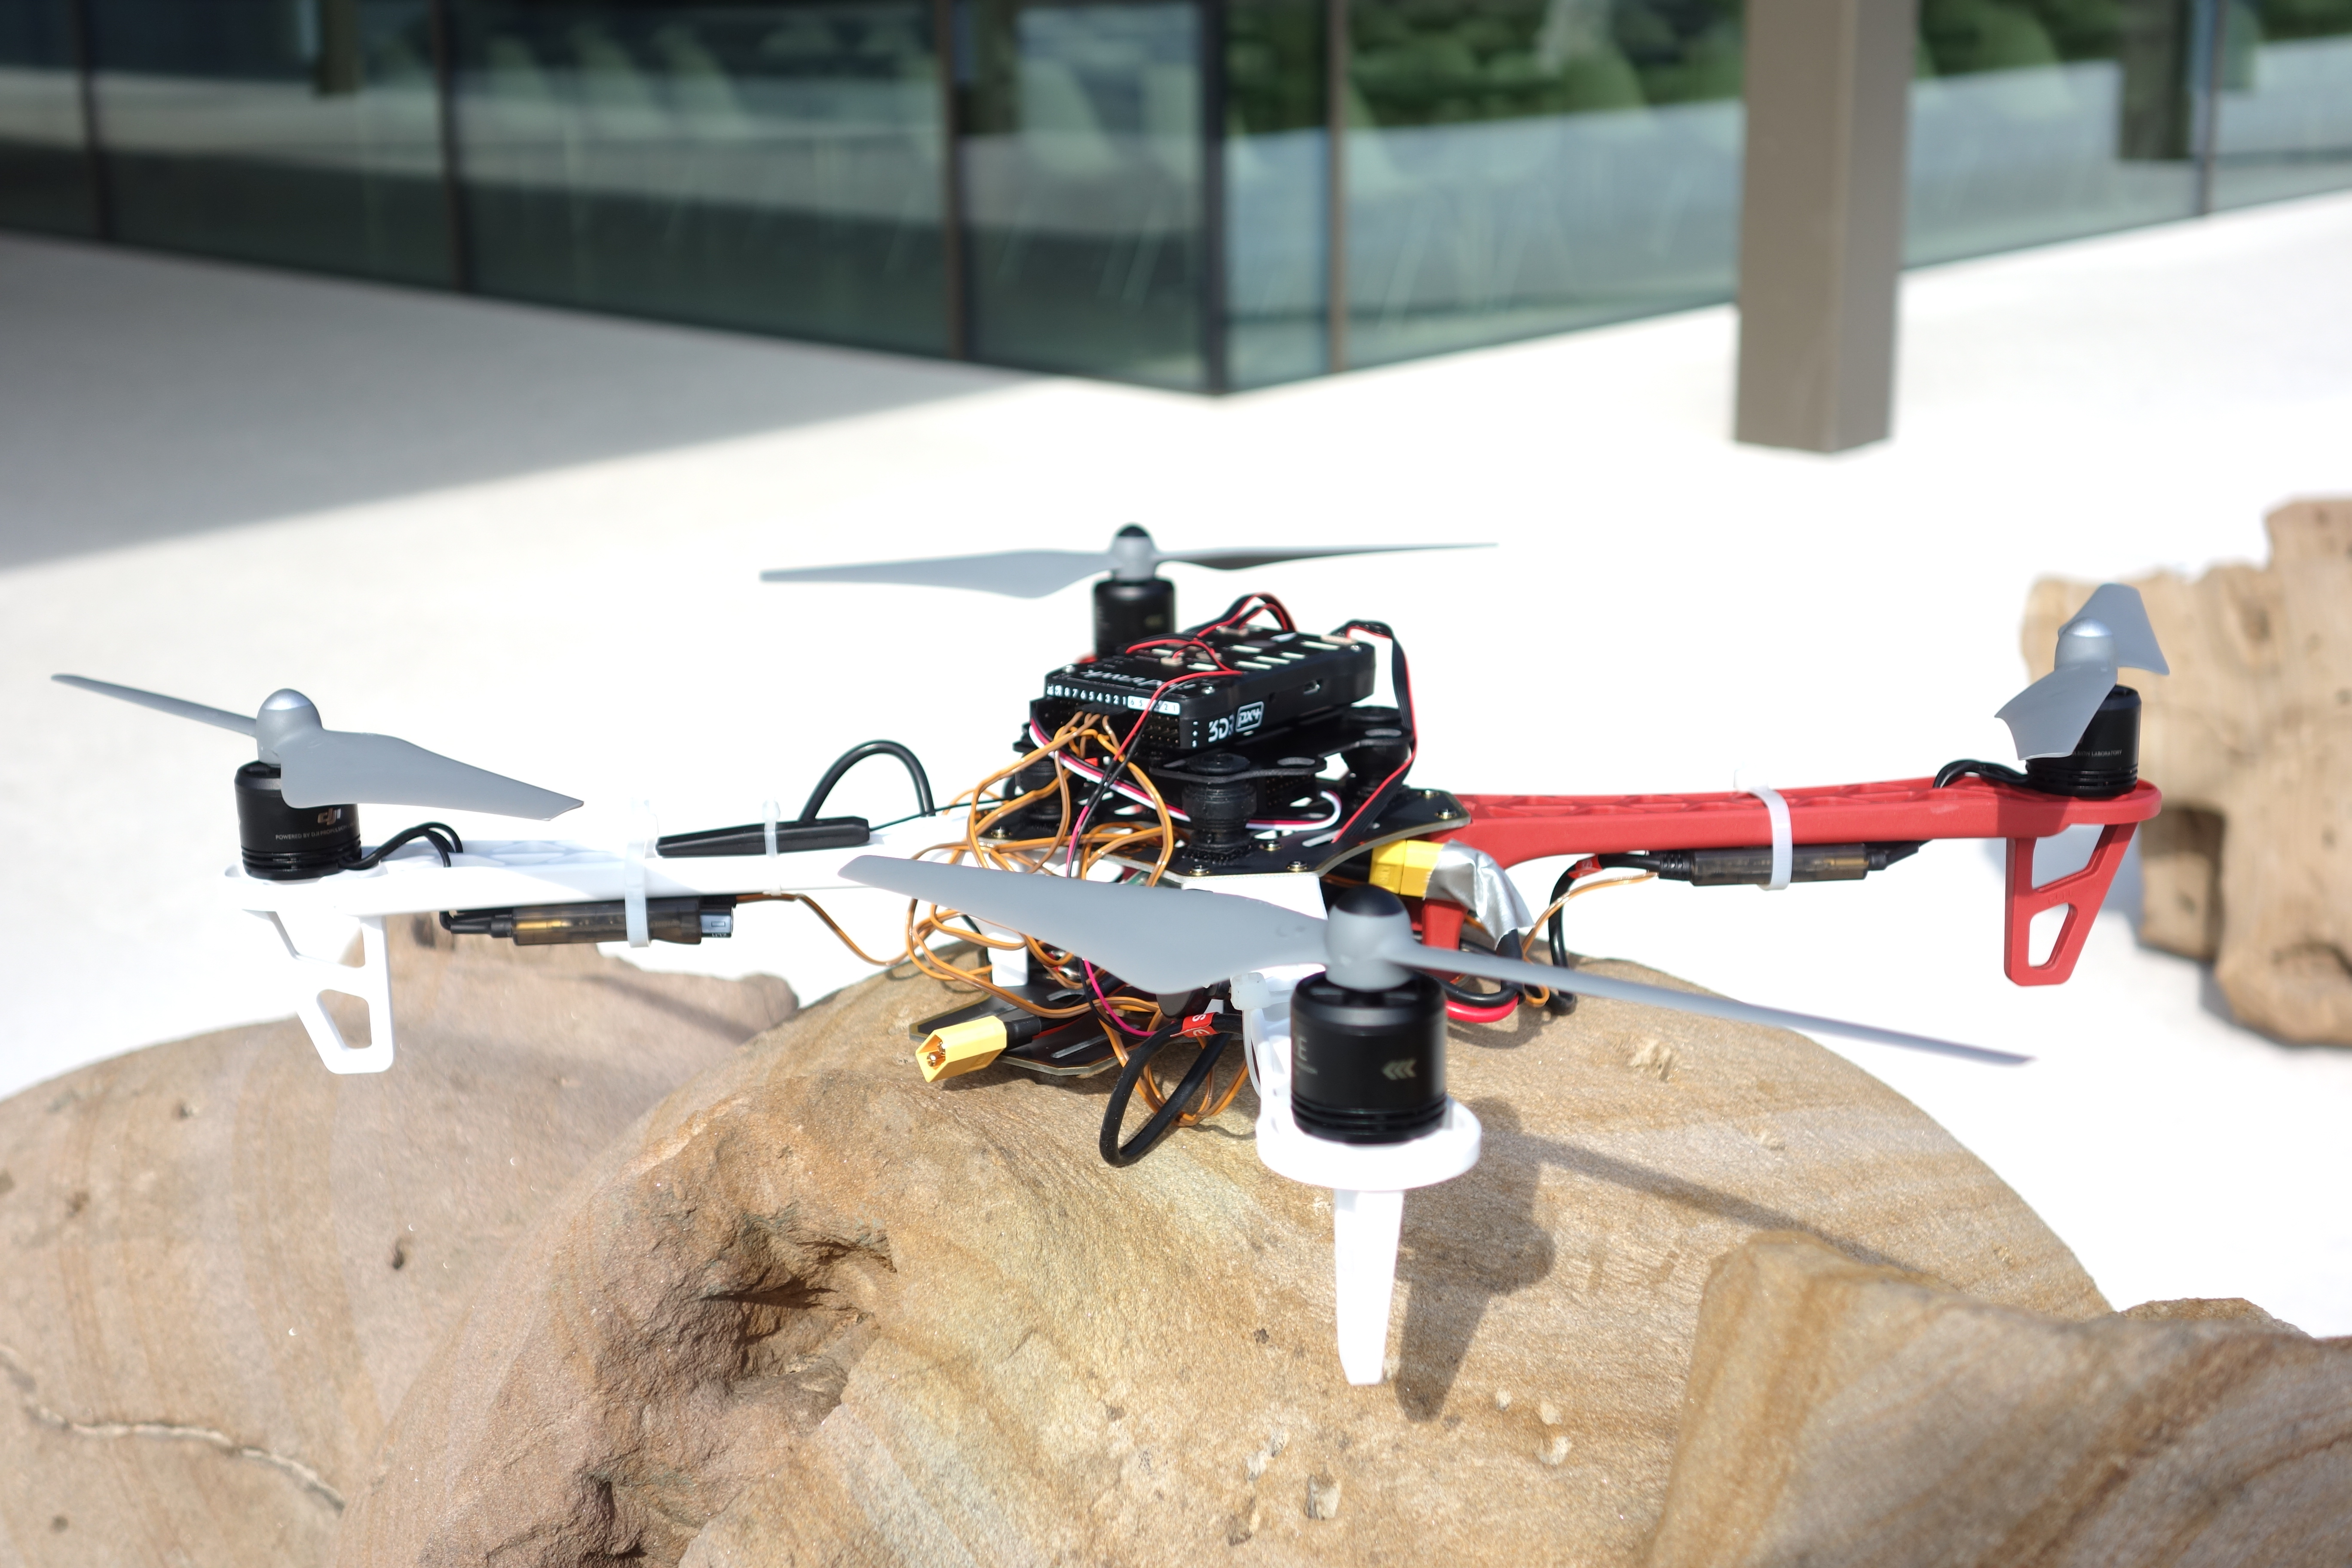
\includegraphics[width=0.4\textwidth] {images/hardware/prototype1.jpg}
\caption{Erster Prototyp ohne Landegestell und ohne Smartphone}
\label{fig:prototyp-1}
\end{figure}

Um das Zusammenspiel der Hardwarekomponenten zu testen und erste Erfahrungen mit dem GPS und den verschiedenen Flugmodi zu sammeln, wurde in der ersten Iteration nur die Drohne in einem minimal Flugzustand aufgebaut.

\subsubsection{Version 2}

\begin{figure}[H]
\centering
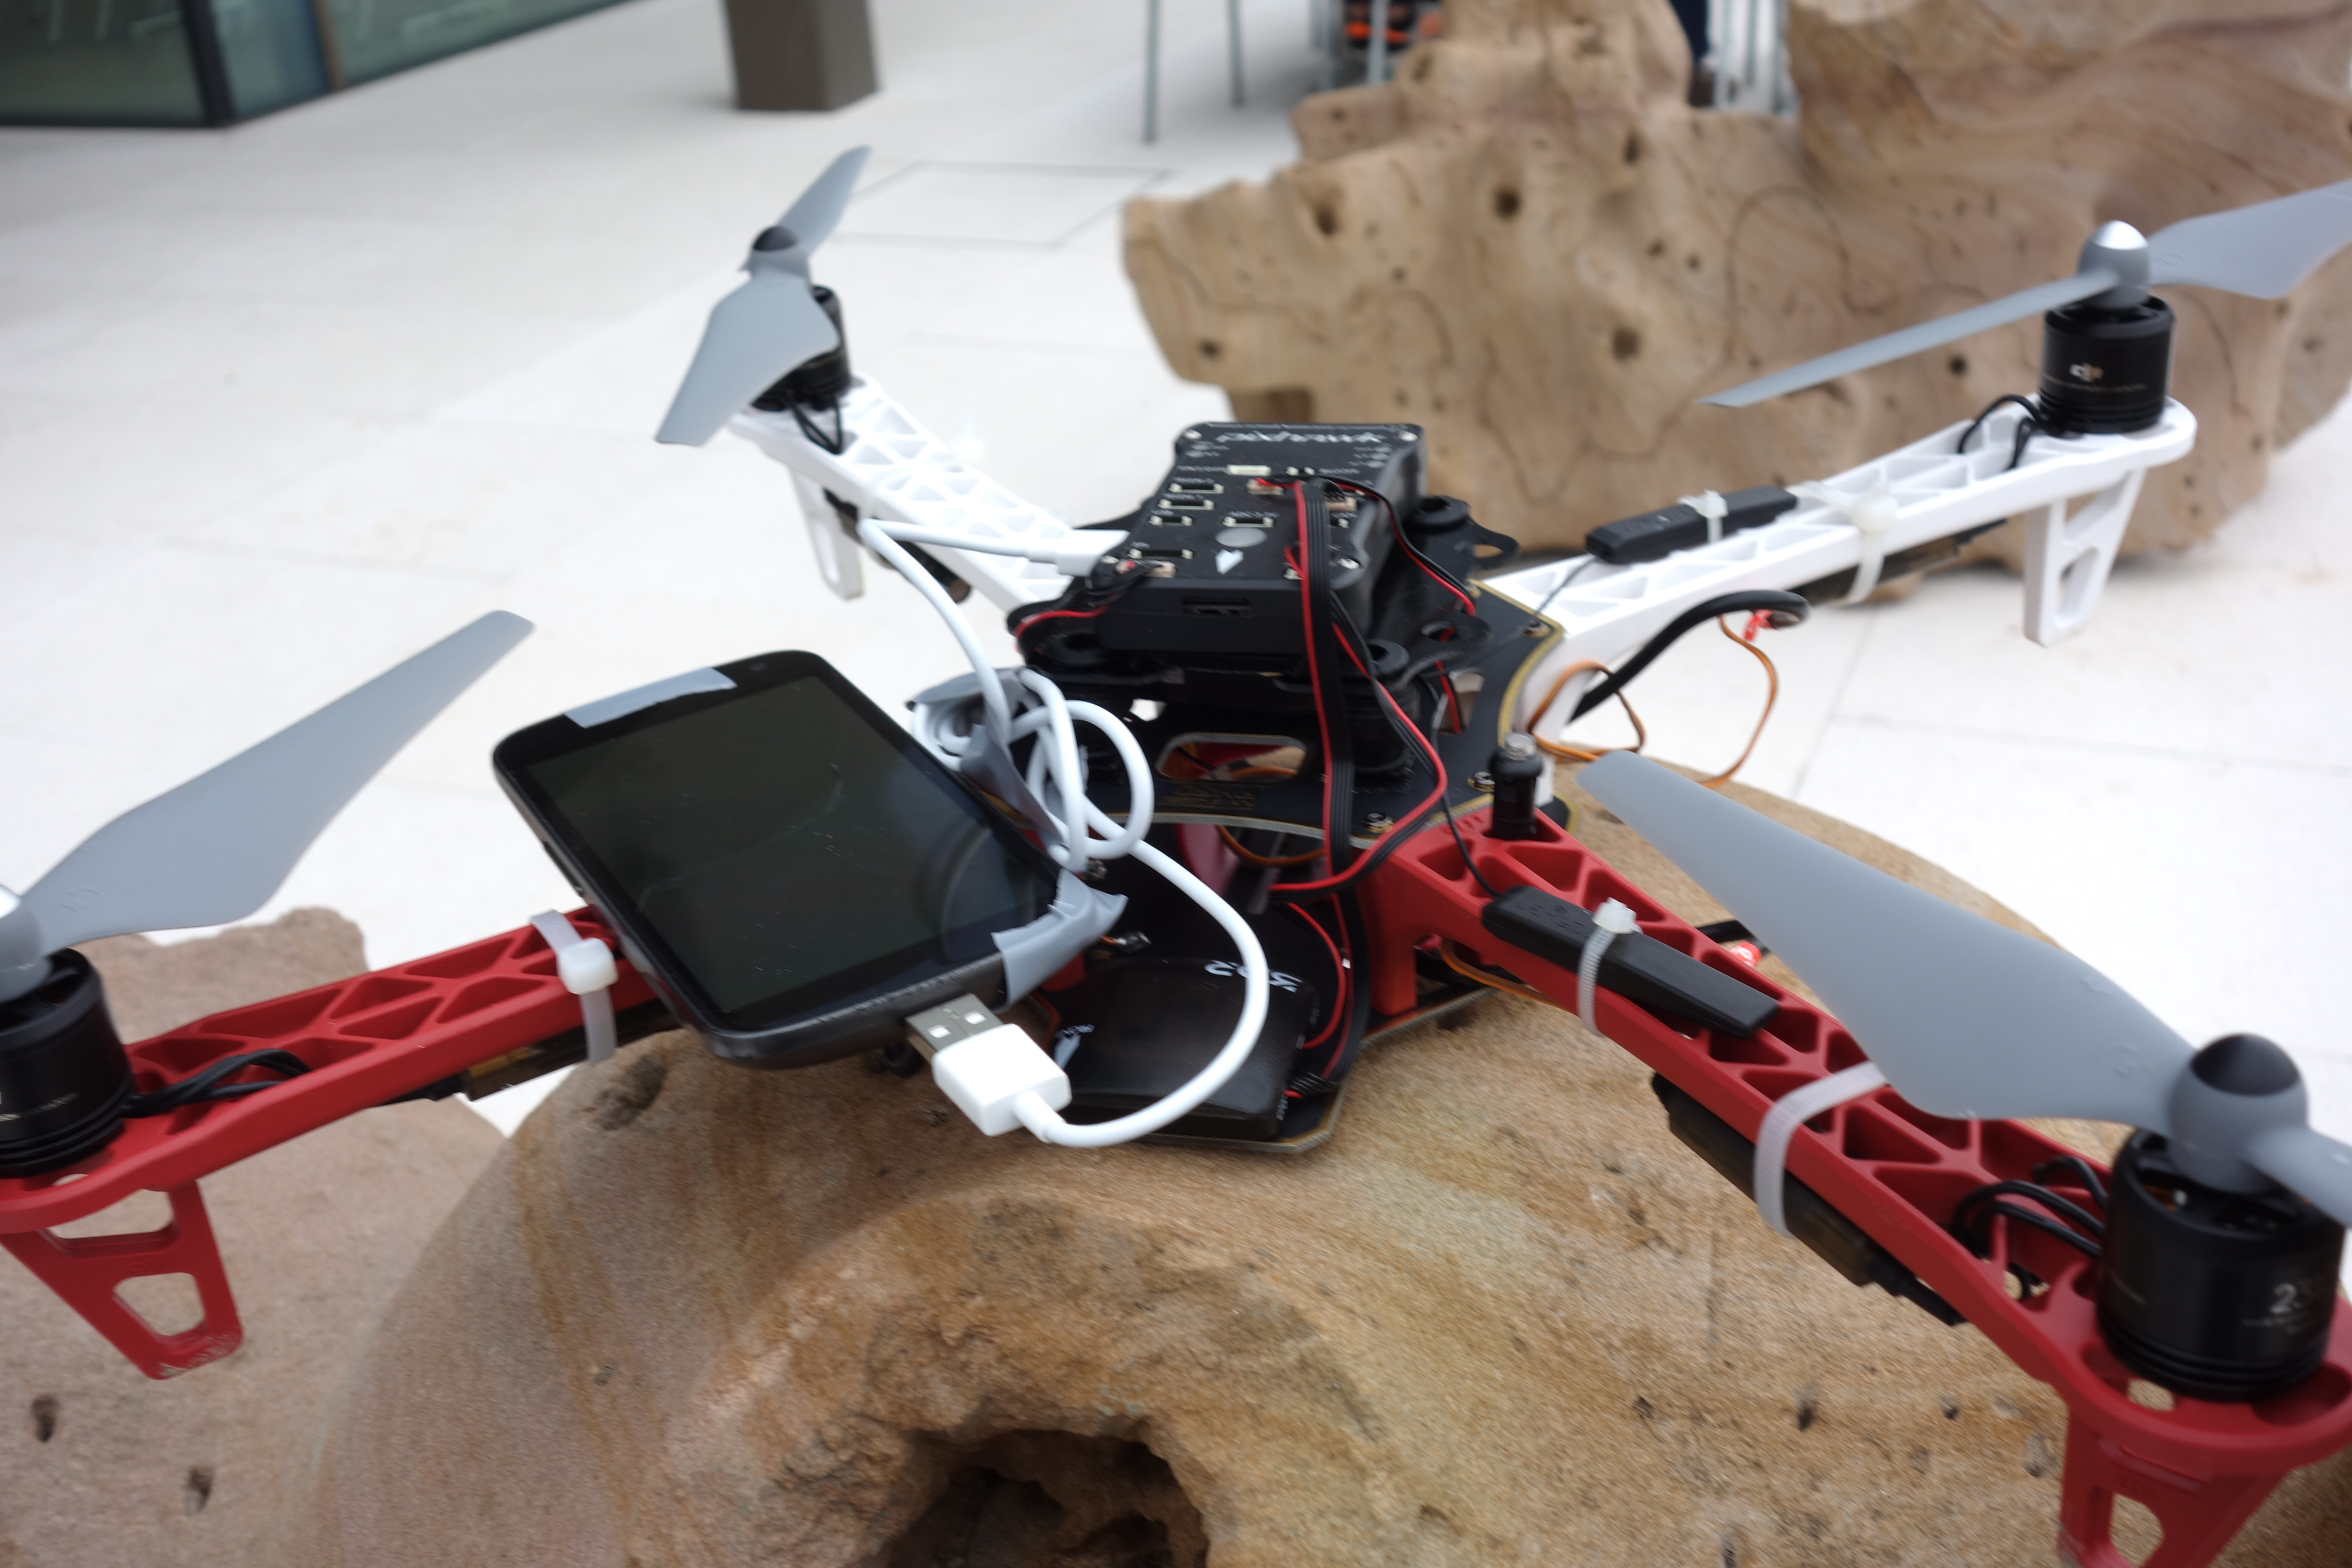
\includegraphics[width=0.4\textwidth] {images/hardware/prototype2.jpg}
\caption{Drohnen Aufbau mit Smartphone}
\label{fig:prototyp-2}
\end{figure}

Um die Risiken R08 (Ardupilot Handhabung) und R09 (Ardupilot API) frühzeitig auszuschliessen (siehe Tabelle \ref{table:risk-table}), wurde das Smartphone zusätzlich auf die Drohne montiert, und mit einem ersten Prototypen der Onboard-App getestet. \\
Nach dem Test wurde uns klar, dass eine Befestigung für das Smartphone erarbeitet werden mussten, um es sicher zu transportieren und bedienbar zu positionieren.

\begin{figure}[H]
	\centering
	\begin{minipage}[b]{0.4\textwidth}
		% TODO Ein Bild ohne Tastatur und Stuhl wäre auch gut?
		\includegraphics[width=\textwidth]{images/hardware/drone-with-handy.jpg}
	\caption{Modell der Handy Halterung}
	\label{fig:case-model}
	\end{minipage}
	\hfill
	\begin{minipage}[b]{0.4\textwidth}
		\includegraphics[width=\textwidth]{images/hardware/case-model.png}
	\caption{Drohne mit Handy Halterung}
	\label{fig:prototyp-3}
	\end{minipage}
\end{figure}

Es wurde eine Halterung konzipiert \ref{fig:case-model}, welche wir später im 3D-Druck Verfahren produzieren liessen.
Die Handy-Halterung konnte auch gleich genutzt werden, um den Pixhawk-Controller zu verstecken und das GPS Module gut exponiert zu montieren. 

\subsubsection{Version 3}
Nachdem mit der Drohne zahlreiche autonome Testflüge unternommen wurden, musste eine Möglichkeit erarbeitet werden, wie die Lieferung an den Kunden gebracht werden kann.

\begin{figure}[H]
	\centering
	\begin{minipage}[b]{0.4\textwidth}
		\includegraphics[width=\textwidth]{images/hardware/parachute-model.jpg}
		\caption{Halterung}
		\label{asdf}
	\end{minipage}
	\hfill
	\begin{minipage}[b]{0.4\textwidth}
		% TODO Hier muss ein bessers Bild her ( oder Kafferahmen weg photoshoppen )
		\includegraphics[width=\textwidth]{images/hardware/drone-with-servo.jpg}
		\caption{Drohne mit dem Abwurfsmechanismus}
		\label{asdf}
	\end{minipage}
\end{figure}


Es wurde ein einfacher Mechanismus mit einem handelsüblichen Modelbau-Servo konstruiert. Die Abbildung \ref{fig:AbwurfMechanismus} zeigt, wie der Servo den Stift entfernt und so die Ladung freigeben kann. \\
Das Packet, an einem Fallschirm befestigt, wird auf den Stift gehängt und verschlossen und der Fallschirm im dazugehörigen Fallschirmschacht verstaut. Der Servo war mittels einer Fernbedienungstaste kontrollierbar und löste so den Abwurf des Paketes aus. Später haben wir den Servo über einen Softwarebefehl auslösbar gemacht. 

\subsection{Kommunikationshardware}
Da die Drohne gemäss unseren Anforderungen eine Verbindung zum Server benötigt, muss geeignete Kommunikationshardware installiert werden. Aus folgenden Gründen haben wir uns für ein Android fähiges Mobiltelefon entschieden:
\begin{itemize}
	\item{Android als Softwareplattform ermöglicht uns die Entwicklung in Java}
	\item{Ein User Interface und Statusanzeige kann auf dem App implementiert werden}
	\item{Es existiert eine passende Bibliothek für die Kommunikation über MAVLink}
	\item{Das Betriebssystem übernimmt den gesammten Kommunikationsstack - sei es im Gebäude mittels WLAN oder im Feld über GSM}
\end{itemize}
Für Verwendungszwecke ohne den Bedarf eines User Interfaces kann man sich allenfalls auch überlegen andere Komponenten zu verwenden. Wir haben 2 Optionen genauer angeschaut und bewertet:
\begin{itemize}
	\item{\textbf{Raspbery PI} \\
	Bereits ab dem leichtgewichtigen Raspberry PI zero sind die nötigen Funktionen vorhanden. Zusätzlich muss hier auf ein GSM Modem zurückgegriffen werden um eine permanente Internetverbindung aufzubauen. Bei Verwendung eines Raspberry PI 3 kann sogar auf ein WLAN Interface zugegriffen werden.
	}
	\item{\textbf{Arduino} \\
	Bei der Arduino Hardware Plattform kann auf einem beliebigen Arduino Board implementiert werden, welches als USB Host Device arbeiten kann. Zusätzlich muss ein GSM Shield 2 verwendet werden um eine GSM Verbindung aufbauen zu können.}
\end{itemize}
Aus unserer Sicht stellen die 2 Embedded Systeme durchaus eine alternative dar. Leider verschwindet aber der Komfort die Drohne zu überwachen mittels dem GUI auf der Onboard App. Beide Alternativen müssen zusätzlich über das Boardstromnetz der Drohne betrieben werden, und benötigen zusätzliche Spannungsregler um die gewünschte Betriebsspannung der Hardware zu gewährleisten. Dies kann noch weiter optimiert werden, wenn die Schaltung genügend Dimensioniert ist, um dem Servo eine stabile Stromversorgung zu gewährleisten, so kann ein externes BEC, welches zur Zeit im Einsatz ist, weg fallen.\\

Abschliessend sollte erwähnt werden, dass die permanente Internetverbindung durchaus eine Anforderung ist, die vieles einschränkt. Kann man sich von dieser Anforderung trennen und mit den Konsequenzen leben, so könnte die Drohne in der Ladezone ausschliesslich mit einem WLAN Netz betrieben werden. Dies wiederum würde einen Raspberry PI 3 sehr attraktiv für dieses Szenario machen.
 
\subsection{Tests}
Um die Anwendungsmöglichkeiten eines solchen Multicopters auszuloten wurden diverse Experimente durchgeführt um die Leistungsfähigkeit und die Einschränkungen zu testen. 

\subsubsection{Akku Laufzeittest}
Um die maximale Akku Laufzeit zu testen wurde die Drohne ohne zusätzliches Gewicht gestartet, etwa 1.5m über dem Boden schweben gelassen und die Zeit gemessen. Dabei versucht die Drohne die Postion zu halten, bei Abweichung wurde aktiv korrigiert. \\

\begin{tabularx}{\textwidth}{|c|c|X|}
\hline
\textbf{Akku} & \textbf{Zuladung} & \textbf{Laufzeit} \\ \hline \hline 
3S & keine & 16min 29s\\ \hline 
2x 4S & 500g & 19min\\ \hline 
\end{tabularx}
\newpage
\subsubsection{Tragfähigkeitstests}
Um das maximale Gewicht zu prüfen, welches auf unsere Drohnen geladen werden kann, wurden Tests mit dem Zielgewicht von ca. 500g durchgeführt. Dies Entspricht dem Gewicht einer PET-Flasche eines beliebigen Getränkeherstellers oder einem leichten Defibrilator. Ausserdem war das Mobiltelefon (ca. 150g) während der Tests auf der Drohne angebracht.  \\

\begin{tabularx}{\textwidth}{|c|c|c|c|X|}
\hline
\textbf{Nutzlast} & \textbf{Akku Typ} & \textbf{Nötige Leistung }& \textbf{Erwartete Flugzeit } & \textbf{Subjektives Flugverhalten }\\
\hline \hline
500g & 3S & ca. 75\%  & n.A. & Ziemlich Träge, mehr Gewicht wäre kritisch\\\hline
500g & 4S & ca. 45\%  & n.A. & Gewicht kaum Spürbar\\
\hline
\end{tabularx}\\

Auch mit 3S Akkus ist es also möglich eine PET-Flasche zu transportieren. Allerdings empfehlen wir für Gewichte über 300 4S-Akkus zu verwenden.\\

Aus den Tragfähigkeitstests schliessen wir, dass auch ein Defibrilator (siehe Aufgabenstellung) mit einer von uns erstellten Drohne transportierbar ist.
\blockquote{I identified the two lightest weight defibrillators on the market in the U.S. at the time of the exploration (March 2013): the Schiller FRED EasyPort (600 grams) and the HeartSine samaritan PAD 300P (1100 grams). The former model is not designed for layperson use, but is far and away the lightest defibrillator available.} 
\cite[p.3]{FleckUAV}
%TODO Zitatdarstellung richtig machen


\section{Ablieferungskonzept}

Um ein möglichst sicheres und einfaches Ablieferungsverfahren zu finden, wurden folgende Optionen in Betracht gezogen.

\subsection{Landung ohne automatischen Abwurf}

Bei diesem Konzept landet die Drohne an der Position des Kunden und dieser kann dann selbst das Paket von der Drohne lösen. Er wird dann mit Hilfe der Onboard-App aufgefordert den Erhalt der Bestellung zu bestätigen. Nach der Bestätigung startet die Drohne einen Countdown, hebt danach ab und fliegt zur Ausgangsposition zurück. Der Kunde kann den Countdown unterbrechen und erneut starten.

Vorteile:
\begin{itemize}
	\item Kunde bestätigt Lieferung
	\item Ware kann keinen Schaden nehmen
	\item Kunde kann entscheiden wann es sicher genug ist, damit die Drohne starten kann.
\end{itemize}


Nachteile:
\begin{itemize}
	\item Drohne kann Personen verletzen, während sie sich in Bodennähe befindet
	\item Aufwendiges Handling auf der Onboard-App
	\item Landung kann schwierig sein je nach Gelände
	\item Fremde Personen haben physischen Zugriff auf die Drohne
\end{itemize}

\subsection{Landung mit automatischem Abwurf}

Dieses System ermöglicht es ohne Fallschirm die Ware abzuwerfen. Dabei Landet die Drohne, löst die Ladung und startet sofort wieder. Es gibt keinerlei Interaktion mit dem Kunden.

Vorteile:
\begin{itemize}
	\item Ware kann keinen Schaden nehmen
\end{itemize}


Nachteile:
\begin{itemize}
	\item Drohne kann Personen verletzen, während sie sich in Bodennähe befindet
	\item Landung kann schwierig sein je nach Gelände
	\item Fremde Personen haben physischen Zugriff auf die Drohne
\end{itemize}


\subsection{Abwurf mit Fallschirm}

Dabei wird ein Fallschirm an der Ware befestigt. Die Drohne löst die Ladung in einer vorgegebenen Höhe und die Ladung schwebt zu Boden.

%TODO Martin hinzufügen Fallschirmberechnungen

Vorteile:
\begin{itemize}
	\item Drohne kann niemanden Verletzen 
	\item Drohne ist ausser Reichweite von Personen
	\item Einfaches Handling auf der Onboard-App
	\item Mechanismus erlaubt auch Landung mit automatischem Abwurf
\end{itemize}


Nachteile:
\begin{itemize}
	\item Ware kann Schaden nehmen
	\item Ware kann Personen verletzen bei Versagen des Fallschirms
	\item Einweg Fallschirme (Kosten und Abfall)
\end{itemize}


\subsection{Entscheidung}

Die Nutzwertanalyse in Abbildung \ref{fig:nutzwertanalyse_abwurf} zeigt klar, dass die letzte Variante die meisten Vorteile bringt. Wichtig ist auch, dass ein Abwurf im gelandeten Zustand weiterhin möglich bleibt, ohne die mechanischen Komponenten zu verändern. Deshalb haben wir uns für einen Abwurf mit dem Fallschirm entschieden.

\begin{figure}[h]
	\centering
	\includegraphics[width=0.9\textwidth] {images/nutzwertanalyse_abwurf.png} 
	\caption{Nutzwertanalyse der verschiedenen Liefervarianten}
	\label{fig:nutzwertanalyse_abwurf}
\end{figure}

\section{Alternative Drohnenarten}

Grundsätzlich können, über das von uns verwendete \Gls{MAVLink} Protokoll, alle Arten von Drohnen angesteuert werden. Beispielsweise bietet die Autopilot-Software \ref{fig:arduScreenshot} 'ArduPilot' Firmware-Varianten für Multicopter, Flugzeuge, Fahrzeuge. \\
\begin{figure}[H]
\centering
\includegraphics[width=0.8\textwidth] {images/arduScreenshot.jpg}
\caption{Screenshot der verschiedenen Firmwarevarianten.}
\label{fig:arduScreenshot}
\end{figure}

Uplift \ref{fig:uplift} Aero beispielsweise war ein Startup, dass versucht hat, Hilfsgüter mit Hilfe von Drohnen von der Türkei aus nach Syrien zu fliegen. Sie haben für ihre Flugzeuge die selben Flugcontroller wie wir verwendet und mussten lediglich die passende Firmware aufspielen. Dies beweist wie flexibel und vielseitig die von uns eingesetzte Hardware verwendet werden kann.

\begin{figure}[H]
\centering
\includegraphics[width=0.8\textwidth] {images/SyriaUplift.jpg}
\caption{Uplift Team und die Syrien-Drohne Quelle: \protect\url{http://uplift.aero/}}
\label{fig:uplift}
\end{figure}



\chapter{Zusammenfassung und Ausblick}

\section{Impressionen der Ergebnisse}

Um den Einstieg für die Zielgruppe zu erleichtern, wurde eine Webseite erstellt, die die wichtigsten Funktionen erklärt und eine Übersicht über die Funktionsweise der Plattform bietet.

\begin{figure}[H]
	\centering
	\includegraphics[width=1\textwidth] {images/website.png}
	\caption{Ausschnitt der Webseite \url{https://my.helin.ch/}}
\end{figure}
\newpage

Ausserdem wurde die Plattform auf \url{https://my.helin.ch/} freigeschaltet und kann frei genutzt werden.

\begin{figure}[H]
	\centering
	\includegraphics[width=1.0\textwidth] {images/myhelin.png}
	\caption{Drohnenliste von MyHelin}
\end{figure}

Die \Gls{Single-Page-Applications} für das Zeichnen von Zonen, das Testen eines Zonensetups und die Überwachung der Lieferungen stehen dann sofort zur Verfügung.

\begin{figure}[H]
	\centering
	\includegraphics[width=1.0\textwidth] {images/map-ui.png}
	\caption{Kartenansicht bei der Verfolgung einer Drohne während der Mission}
\end{figure}

\newpage
Das Customer-App für Android (links), das Customer-App für iOS (mitte) und das Onboard-App (rechts) können verwendet werden.

\begin{figure}[H]
	\centering
	\begin{minipage}[b]{0.2\textwidth}
			\centering
		\includegraphics[width=\textwidth]{images/customer-app-android.png}
		\label{fig:customer-app-android}
	\end{minipage}
	\hfill
	\begin{minipage}[b]{0.2\textwidth}
		\centering
		\includegraphics[width=\textwidth]{images/customer-app-ios.png}
		\label{fig:customer-app-ios}
	\end{minipage}
	\hfill
	\begin{minipage}[b]{0.2\textwidth}
			\centering
		\includegraphics[width=\textwidth]{images/onboard-app.png}
		\label{fig:onboard-app-android}
	\end{minipage}
\end{figure}


Die Drohne zusammen mit dem Onboard-App konnte auf einen Stand gebracht werden, mit dem sie mehrere Lieferungen hintereinander ohne Schwierigkeiten ausführen kann.

\begin{figure}[H]
	\centering
	\includegraphics[width=1.0\textwidth] {images/parachute-test.jpeg}
	\caption{Diverse erfolgreiche Tests mit dem autonomen Abwurf der Ladung}
\end{figure}

\begin{figure}[H]
	\centering
	\includegraphics[width=0.95\textwidth] {images/drone-drop.jpg}
	\caption{Liefertest mit einem Verbandskasten}
\end{figure}
\begin{figure}[H]
	\centering
	\includegraphics[width=0.95\textwidth] {images/drone-drop2.jpg}
	\caption{Liefertest nach dem Öffnen des Fallschirms}
\end{figure}


\begin{figure}[H]
	\centering
	\includegraphics[width=1.0\textwidth] {images/drone.jpg}
	\caption{Drohne mit Onboard-App in der finalen Ausbaustufe}
\end{figure}


\newpage
\subsection{Zusammenfassung der Ergebnisse}

Während dieser Arbeit hat das Team eine Plattform konzipiert und entwickelt, die es jedem Anbieter ermöglicht, einen autonomen Drohnen-Lieferservice für ein von ihm definiertes Gebiet aufzubauen. Die Plattform wurde auf einem Server als Software as a Service zur Verfügung gestellt. Ausserdem wurde der gesamte Code des Projekts auf GitHub veröffentlicht und steht unter einer \Gls{MIT-Lizenz} als Open Source Software zur Verfügung. Die Tests mit den zwei eigens aufgebauten Drohnen zeigen, dass das System als Ganzes funktioniert. \\

Folgende Ergebnisse sind besonders hervorzuheben:

\begin{itemize}
	\item Webseite für Administratoren zur Verwaltung von Organisationen, Drohnen, Produkten und Bestellungen
	\item Cross-Plattform Bestell-App (iOS, Android) für Kunden
	\item Android App zur Steuerung der Drohne über das Internet
	\item Verfolgung der Drohnen-Telemetrie während, vor und nach der Lieferung einer Bestellung
	\item Automatisierte dynamische Routenberechnung über vordefinierte Flugzonen, abhängig von der Position des Kunden
	\item Automatisierte Verteilung von Lieferaufträgen an die Drohnen
	\item Getestete Vorlage für den Aufbau einer Lieferdrohne
	\item Vorgefertigte 3D-Modelle für den 3D-Druck der Smartphone-Halterung und der Abwurfvorrichtung
\end{itemize}

\newpage
\section{Ausblick}

Die entwickelte Plattform zeigt erst einen Bruchteil der Möglichkeiten, die in Zukunft von autonomen Drohnen übernommen werden können. Beispielsweise können Videoaufnahmen, Infrastruktur-Überwachung oder Katastrophenhilfe als Angebote integriert werden. 

\subsection{Empfohlene Weiterentwicklungen}

Während des Projekts sind weitere Ideen entstanden: 

\subsubsection{Plattform}

\begin{itemize}
	\item Services hinzufügen (Drone-Selfie, Follow-Me Video, geographische Vermessung)
	\item Aktion am Zielort wählbar oder vom Produkt abhängig machen
	\item Test, ob es auch mit Radio-Telemetry am Onboard-App funktioniert
	\item \Gls{Flight-Controller} ohne \Gls{MAVLink} auch unterstützen (z.B. DJI-Onboard-SDK \cite{dji-sdk})
	\item Globale Flugzonen die in allen Projekten sichtbar sind
	\item Kollisionsvermeidung von Drohnen auf denselben Routen
	\item Objekte mit Kollisionspotential (z.B. Gebäude, Bäume) automatisiert aus Flugzonen ausschliessen
\end{itemize}

\subsubsection{Drohnen Hardware} 
\begin{itemize}
	\item Testen in Kombination mit Obstacle Avoidance (z.B. Intel RealSense\cite{realsense}) Hardware
		\item Tests mit anderen Arten von Drohnen (siehe Abschnitt \ref{sec:drone-alternatives})
	\item Smartphone ersetzen durch Embedded-System (siehe Alternativen im Abschnitt \ref{sec:communication-architecture}) 

	\item Automatisches Beladungssystem für Drohnen
	\item Automatisches Batterieaustauschsystem für Drohnen
\end{itemize}  



\subsection{Known-Issues}

Alle bekannten kleineren Probleme und zusätzlichen Features, die vor einem produktiven Einsatz des Systems umgesetzt werden sollten, werden im Server-GitHub-Repository als Issues erfasst. Dies ermöglicht es auch anderen Entwicklern an dem Projekt weiterzuarbeiten und dessen Limitierungen zu kennen.

\newpage
\section{Schlussfolgerung}

Während dieser Arbeit haben wir aus unserer Vision ein Produkt entwickelt und fertiggestellt. Damit konnten wir beweisen, dass man mit verfügbaren Technologien Liefersysteme mit autonomen Drohnen schon heute realisieren kann. Die entstandene Plattform kann nun zu Testzwecken von allen Interessierten genutzt und weiterentwickelt werden.\\

Die erarbeiteten funktionalen- und nicht-funktionalen Anforderungen konnten alle erfüllt und teilweise übertroffen werden, trotz der vielfältigen und teilweise interdisziplinären Aufgaben, die dieser Arbeit innewohnten. \\

Unserer Meinung nach ist unsere Plattform ein Beispiel für die Drohnen-Projekte der Zukunft. Vor allem in Bezug auf die Verwendung einer zentralen Instanz, zur Steuerung und Überwachung einer Drohnenflotte. Dadurch gewinnen viele Projekte, wie das Überwachen von Haien \cite{shark}, die Lieferung von Defibrillatoren \cite{defibrillator-drone} oder das Finden von Überlebenden in einem Katastrophengebiet \cite{catastrophic-drone}, deutlich an praktischer Relevanz und können flächendeckend eingesetzt werden. Wir hoffen, dass die entwickelte Plattform als Anstoss für die Stakeholder in dieser Branche dienen kann und sich die Technologien und Gesetzeslagen insoweit verbessern, dass Dienstleistungen von autonomen Drohnen bald für eine grössere Anzahl von Kunden zur Verfügung stehen werden.







\part{Anhang}
\newpage
\renewcommand \thechapter{\Alph{chapter}}

\newpage

\chapter{Infrastruktur}

\section{Server}

Für die Helin Applikation steht ein Server bereit. Wie in der Abbildung \ref{fig:communication-architecture-overview} dargestellt, wird dieser als Build-, Test- und Applikations-Server verwendet. 
Auf dem Server läuft eine PostgreSQL Datenbank mit einer PostGIS Extension, welche für die Routenberechnung benötigt wird. Gleichzeitig ist ein RabbitMQ-Message-Broker und eine Instanz der Helin Server Applikation installiert. Aus Resourcengründen wird alles auf einem Server ausgeführt, könnte aber bei Leistungsproblemen ohne weiteres auf mehrere Server verteilt werden. Als Build- und Test-Server für alle Applikationen wird TeamCity verwendet. 

Neben dem Server werden auch Apps für Android Geräte veröffentlicht. Beide kommunizieren primär mit der RabbitMQ Instanz auf dem Server.

\begin{figure}[h]
	\includegraphics[width=1.0\textwidth]{images/DeploymentDiagram.png}
	\caption{Deployment Diagram}
	\label{fig:deployment-diagram}
\end{figure}




\definecolor{boxred}{RGB}{234,99,99}
\definecolor{boxorange}{RGB}{255,242,204}
\definecolor{boxgreen}{RGB}{217,234,211}

\newcommand{\greenbox}{
\begin{tikzpicture}
\draw[line width=0pt, fill=boxgreen]
(0, 0) rectangle (0.3, 0.3);
\end{tikzpicture}}

\newcommand{\orangebox}{
\begin{tikzpicture}
\draw[line width=0pt, fill=boxorange]
(0, 0) rectangle (0.3, 0.3);
\end{tikzpicture}}

\newcommand{\redbox}{
\begin{tikzpicture}
\draw[line width=0pt, fill=boxred]
(0, 0) rectangle (0.3, 0.3);
\end{tikzpicture}}

\chapter{Projektplan}
\section{Änderungsgeschichte}
\begin{tabularx}{\textwidth}{|c|c|X|c|}
  \hline
  \textbf{Datum} & \textbf{Version} & \textbf{Änderung} & \textbf{Autor} \\
  \hline \hline
  26.02.2016 & 1.0 & Erstellen des Projektplans & Martin Stypinski \\
  11.03.2016 & 1.1 & Risiken nach Sprint 1 & Marcel Amsler \\
  26.03.2016 & 1.2 & Risiken nach Sprint 2 & Kirusanth Poopalasingam \\
  12.04.2016 & 1.3 & Risiken nach Sprint 3 & Marcel Amsler \\
  28.04.2016 & 1.4 & Risiken nach Sprint 4 & Kirusanth Poopalasingam \\
  04.06.2016 & 1.5 & Risiken nach Sprint 5 & Martin Stypinski \\
  11.06.2016 & 1.6 & Verantwortlichkeiten dokumentiert & Marcel Amsler \\
  11.06.2016 & 2.0 & Finalisieren des Projektplans & Martin Stypinski \\
  \hline
\end{tabularx}

\section{Einleitung}
\subsection{Ziel und Zweck}
Ziel dieser Arbeit ist es, eine Web-Applikation zu entwickeln, die es ermöglicht Drohnenflotten zu verwalten und damit vollautomatisierte Lieferungen auszuführen. Nutzer dieser Applikation können dazu Flugzonen definieren, in denen ein sicherer Flug von Drohnen möglich ist. Kunden hingegen sollen durch eine App die Möglichkeit erhalten, Güter zu bestellen, welche an ihre aktuelle Position ausgeliefert werden.

\subsection{Lieferumfang}
Der Lieferumfang dieser Arbeit entspricht den Vorgaben der HSR:
\begin{itemize}
	\item{Zu Handen des Betreuers:
	\begin{itemize}
		\item{Ein gedrucktes Exemplar der Dokumentation}
		\item{Dokumentation, sämtliche Dokumente und Sourcen auf CD}
	\end{itemize}}
	\item{Poster - Enthält Zusammenfassung der Arbeit}
	\item{Abstract für die Bachelorarbeitsbrochure}
\end{itemize}
Zusätzlich ist es uns ein Anliegen, dass der Sourcecode und die Erfahrungen über den Zeitraum der Bachelorarbeit hinaus bestehen bleiben. Daher wurde ein GitHub-Repository eingerichtet, dass nach Beendigung der Arbeit sämtliche Teile enthält: \textbf{\url{https://github.com/Project-Helin}}

\subsection{Annahmen und Einschränkungen}
Es kann angenommen werden, dass der Zeitplan im Rahmen der regulären Bachelorarbeit Zeit gültig ist. Es wird dabei berücksichtigt das ein Zeithorizont von 17 Wochen zur Verfügung steht und die maximale Arbeitszeit von 360 Stunden pro Person nicht überschritten werden soll.
\section{Projektorganisation}
\subsection{Organisationsstruktur}
\begin{figure}[ht]
%\begin{figure}[H]
	\centering
	\includegraphics[width=\textwidth]{images/organigram.png}
	\caption{Grobübersicht über den Projektplan}
	\label{Risk result}
\end{figure}
\noindent
\begin{tabularx}{\textwidth}{|c|c|X|}
  \hline
  \textbf{Name} & \textbf{E-Mail} & \textbf{Verantwortung} \\
  \hline \hline
  Prof. Dr. Markus Stolze & \url{markus.stolze@hsr.ch} & Betreuer der Arbeit\\
  \hline \hline
  Marcel Amsler & \url{marcel.amsler@hsr.ch} & \\
  \hline
  Kirusanth Poopolasingam & \url{kirusanth.poopalasingam@hsr.ch} & \\
  \hline
  Martin Stypinski & \url{martin.stypinski@hsr.ch} & \\
  \hline
\end{tabularx}
\newpage

\subsection{Verantwortlichkeiten}
Die Verantwortung und eine Unterstüzungsfunktion für alle Hauptkomponenten haben wird zu beginn der Arbeit folgendermassen festgelegt.\\

\begin{tabularx}{\textwidth}{|c|c|c|c|X|}
	\hline
	\textbf{} & \textbf{Server CRUD} & \textbf{Server Javascript} & \textbf{Onboard-App} & \textbf{Customer App} \\
	\hline \hline
	Hauptverantwortung & KP & MS & MA & MA\\
	\hline \hline
	Unterstützung & MS & MA & MS & KP \\
	\hline
\end{tabularx}\\

KP = Kirusanth Poopalasingam, MA = Marcel Amsler, MS = Martin Stypinski
\newpage


\subsection{Meetings}
In der Regel wird ein Meeting jeweils am Donnerstag um 10.30 in der Mensa abgehalten. In Ausnahmefällen können die Termine von der Planung abweichen.
  \\[1\normalbaselineskip]
\begin{tabularx}{\textwidth}{|c|c|c|X|}
  \hline
  \textbf{SW} & \textbf{Datum} & \textbf{Zeit} & \textbf{Art der Sitzung} \\
  \hline \hline
  1 & 25.02.2016 & 10:00 - 11:00 &  Kick-off meeting \\
  2 & 03.03.2016 & 15:00 - 16:00 &  Meeting mit Betreuer \\
  3 & 10.03.2016 & 10:30 - 11:30 &  Meeting mit Betreuer \\
  4 & 17.03.2016 & 11:00 - 11:45 &  Meeting mit Betreuer \\
  5 & 24.03.2016 & 10:30 - 11:30 &  Meeting mit Betreuer \\
  6 & 08.04.2016 & 13:30 - 14:30 &  Meeting mit Betreuer \\
  7 & 14.04.2016 & 10:30 - 11:30 &  Meeting mit Betreuer \\
  8 & 21.04.2016 & 10:30 - 11:30 &  Meeting mit Betreuer \\
  9 & 28.04.2016 & 11:00 - 11:45 &  Meeting mit Betreuer \\
  9 & 29.04.2016 & 15:00 - 16:00 &  Zwischenpräsentation bei Prof. Beat Stettler \\
  11 & 11.05.2016 & 18:15 - 19:00 &  Zwischenpräsentation bei Thomas Kälin und Prof. Dr. M. Stolze \\
  11 & 12.05.2016 & 10:30 - 11:30 &  Meeting mit Betreuer \\
  12 & 19.05.2016 & 10:00 - 11:00 &  Meeting mit Betreuer \\
  13 & 26.05.2016 & 10:30 - 11:30 &  Meeting mit Betreuer \\
  14 & 02.06.2016 & 10:30 - 11:30 &  Meeting mit Betreuer \\
  15 & 09.06.2016 & 10:30 - 11:30 &  Meeting mit Betreuer \\
  \hline
\end{tabularx}
\newpage
\section{Meilensteinplanung}
Grundsätzlich wird während der gesamten Arbeit Agiles-Projektmanagement mit Scrum als Methode eingesetzt. Ein Scrum-Sprint dauert in der Regel 2 Wochen. Die Meilensteine dienen nur zu Priorisierungszwecken.

\begin{figure}[ht]
%\begin{figure}[H]
	\centering
	\includegraphics[width=\textwidth]{images/projplan.png}
	\caption{Grobübersicht über den Projektplan}
	\label{Risk result}
\end{figure}

\begin{itemize}
	\item{\textbf{Ende Einarbeitung: (MS-1)} 
		\begin{itemize}
			\item{\textbf{Datum:} 11.03.2016}
			\item{\textbf{Ziel:} Entwicklungsumgebung und Prozesse stehen.}
			\item{\textbf{Erfüllungskriterium:} Sämtliche prozessbegleitenden Massnahmen sind lauffähig. Projektmanagement-Tool, IDEs, CI}
		\end{itemize}
	}
	
	\item{\textbf{Ende Proof of Concept: (MS-2)} 
		\begin{itemize}
			\item{\textbf{Datum:} 25.03.2016}
			\item{\textbf{Ziel:} Die Machbarkeit ist bewiesen.}
			\item{\textbf{Erfüllungskriterium:} Prototyp ist lauffähig, zeigt Machbarkeit und allfällige Einschränkungen.}
		\end{itemize}
	}
	
	\item{\textbf{Ende Implementierung: (MS-3)} 
		\begin{itemize}
			\item{\textbf{Datum:} 03.06.2016}
			\item{\textbf{Ziel:} Code Freeze}
			\item{\textbf{Erfüllungskriterium:} Alle zwingenden funktionalen- und nicht-funktionalen Anforderungen sind erfüllt.}
		\end{itemize}
	}	
	\item{\textbf{Abgabe: (MS-4)} 
			\begin{itemize}
				\item{\textbf{Datum:} 17.06.2016}
				\item{\textbf{Ziel:} Abgabe der Arbeit}
				\item{\textbf{Erfüllungskriterium:} Alle im Lieferumfang geforderten Dokumente sind fertiggestellt.}
			\end{itemize}
	}
	
\end{itemize}

\newpage


\begin{landscape}
\section{Risikomanagement}
\subsection{Risiken}
\LTXtable{0.75\paperheight}{risk.tex}
\end{landscape}
\subsection{Umgang mit Risiken}
Die Risken wurden in einer Risiko Matrix aufgegliedert um besser zu verstehen, welche Risiken eine grosse Bedrohung darstellen.

\begin{figure}[ht]
%\begin{figure}[H]
	\centering
	\includegraphics[scale=0.7]{images/risk_result.png}
	\caption{Risiko Matrix}
	\label{Risk result}
\end{figure}

Als Konsequenz der Matrix kann folgende Aufteilung getroffen werden:
\begin{itemize}
	\item{\textbf{Risiko hoch:} R03, R06}
	\item{\textbf{Risiko mittel:} R01, R04, R05, R07, R08, R09, R10, R12 }
	\item{\textbf{Risiko klein:} R02, R11, R13, R14}
\end{itemize}
\subsection{Massnahmen}
Für die Risiken der Kategorie mittel und hoch wurden folgende Massnahmen festgelegt:
\begin{itemize}
	\item{\textbf{R03 - Internet auf Mobilgerät:} \\
	\textbf{Massnahmen:} Es muss sichergestellt werden, dass die Drohne nicht auf eine permanente Serververbindung angewiesen ist. Monitor und Datenlogging dürfen Unterbrechungen aufweisen. Die Mission darf aber zu keinem Zeitpunkt gefährdet werden, die Drohne muss selbstständig ihre Aufgabe erfüllen können und danach wieder zurückkehren.}
	
	\item{\textbf{R06 - Absturz und Schäden:} \\
	\textbf{Massnahmen:} Bei der Wahl der Drohne wurde auf die Verfügbarkeit der Ersatzteile geachtet, sofern dies möglich war. }

	\item{\textbf{R01 - JMS auf Mobilgerät:} \\
	\textbf{Massnahmen:} Bei der Evaluierung der Komponenten wird eine JMS Implementierung gewählt, die auf einem Android Betriebssystem lauffähig ist. Dies wird in einem Proof of Concept überprüft.}
	
	\item{\textbf{R04 - Infrastruktur Probleme:} \\
	\textbf{Massnahmen:} Auf Grund von Erfahrungen aus früheren Projekten, wird auf die Serverinfrastruktur der HSR verzichtet, dies garantiert eine volle Kontrolle über den Server. Es muss jedoch berücksichtig werden, dass der administrative Aufwand höher ist und somit mehr Zeit in Anspruch nehmen wird.}
	
	\item{\textbf{R05 - Kapazität der Drohne:} \\
	\textbf{Massnahmen:} Es werden Güter verwendet, deren Gewicht von der Drohne transportiert werden kann.}	
	
	\item{\textbf{R07 - Positionsungenauigkeit:} \\
	\textbf{Massnahmen:} Bei Flugkorridoren und Landepunkten wird genügend Sicherheitsmarge eingerechnet um die Ungenauigkeit zu relativieren.}
	
	\item{\textbf{R08 - Ardupilot Handhabung:} \\
	\textbf{Massnahmen:}  Im Proof of Concept wird überprüft, wann und wie Updates gemacht werden können. Falls Updates während des Flugs nicht möglich sind, wird von Anfang an die gesamte Route an Ardupilot übertragen.}
	
	\item{\textbf{R09 - Ardupilot API:} \\
	\textbf{Massnahmen:} Früh in einem Proof of Concept die Möglichkeiten und Grenzen des APIs nachvollziehen.}
	
	\item{\textbf{R10 - Entwicklungsprozesse:} \\
	\textbf{Massnahmen:} Es wird während des Proof of Concepts versucht einen Simulator zu verwenden um Zeit zu sparen. Gegebenenfalls Arbeitsplatz im Freien, um Zeit während des Deployments auf die Drohne zu sparen.}
	
	\item{\textbf{R12 - Ablademanagement:} \\
	\textbf{Massnahmen:} Prüfung einer Abwurfmöglichkeit. Gegebenenfalls Benutzer mit GUI auf Mobile begleiten um einen sicheren und unfallfreien Ablad zu garantieren.}
\end{itemize}

\section{Qualitätsmassnahmen}	
\subsection{Dokumentation}
Die Dokumentation wird vollständig in Latex geschrieben und befindet sich zu jedem Zeitpunkt auf dem Project-Helin GitHub-Repository: \url{http:www.github.com/project-helin}. Alle grösseren Änderungen werden immer von einem anderen Teammitglied gelesen und überprüft.

\subsection{Projektmanagement}
Für das Projektmanagement wird Jira von Atlassian verwendet. \\
Als Projektmanagmenet Methodik wird Scrum verwendet, jedoch werden einige Meilensteine gesetzt um den Fokus nicht aus den Augen zu verlieren und sich über Teilziele bewusst zu sein.

\subsection{Entwicklung}
Die Qualität der Entwicklung wird durch folgende Massnahmen sichergestellt:
\begin{itemize}
	\item{\textbf{Code Review:} Bei kritischen Komponenten werden Code Reviews durchgeführt.}
	
	\item{\textbf{Feature Review:} Bei allen Features bzw. umgesetzten User-Stories führt ein anderes Teammitglied eine Qualitätskontrolle durch. Diese kontrolliert hauptsächlich die Erfüllung der Acceptance-Criterias.}
	
	\item{\textbf{Testing:} Das gesammte Projekt wird in Java entwickelt. Als Unit-Test Framework JUnit4 verwendet.}
	
	\item{\textbf{Versionierung:} Der gesammte Quellcode wird mit Hilfe von GitHub versioniert.}
	
	\item{\textbf{Deployment:} Die Serverkomponenten werden mithilfe eines Build Systems deployt. Die Komponenten auf den Mobiltelefonen werden manuell deployt. Jedoch wird auf dem Build-System für alle Komponenten die Ausführung von Unit-Tests garantiert.}
	
\end{itemize}

\newpage

\chapter{Code Standards}
Im Team wurden folgende Code-Conventions eingeführt.

\subsubsection{Autorfreie Klassen}
In Java wird klassischerweise der Autor im Javadoc Kommentar in der Klasse angegeben.

\begin{lstlisting}
/**
 * @author Kirusanth Poopalasingam (pkirusanth@gmail.com)
 */
public class MyTestClass{
}
\end{lstlisting}
Der Autor in der Klasse suggeriert, dass nur ein Autor für diese Klasse existiert und für diese Klasse verantwortlich ist. Dies sollte aber nicht der Fall sein, da jedes Teammitglied verantwortlich für die gesamte Code-Qualität ist und zudem ist die Angabe auf der Klasse heutzutage mit einem Version Control System redundant.

\subsubsection{Javadoc}
Generell sollte Javadoc nur dort verwendet werden, wo es nötig ist. Da es sich bei Projekt Helin nicht um eine API handelt, sollten auch die Methoden und Parameter nicht redundant dokumentiert werden. Ein Beispiel für eine schlechte Javadoc Dokumentation sieht folgendermassen aus:
\begin{lstlisting}
// Beispiel einer Play Klasse
public final class ConfigUtil {
    private ConfigUtil() { }

    /**
     * Quotes and escapes a string, as in the JSON specification.
     *
     * @param s
     *            a string
     * @return the string quoted and escaped
     */
    public static String quoteString(String s) {
        return ConfigImplUtil.renderJsonString(s);
    }
    // ...
}
\end{lstlisting}
Bei der Methode quoteString() kann der ganze Javadoc Kommentar weggelassen werden, da er nicht mehr Aussagekraft hat, als die Methode selbst. Stattdessen sollte die Methode so geschrieben werden, dass die Namen aussagekräftiger sind.
\\
Eine bessere Implementierung würde folgendermassen aussehen:
\begin{lstlisting}
public final class ConfigUtil {
    private ConfigUtil() { }

    public static String quoteStringAccordingToJsonSpecification(String unquotedJson) {
        return ConfigImplUtil.renderJsonString(unquotedJson);
    }
    // ...
}
\end{lstlisting}
\subsubsection{Code}
Für die Formatierung und den Static Check werden die 'Code Inspection' von IntelliJ IDEA verwendet.
\\
Es handelt sich bei den 'Code Inspections' um konfigurierbare Regeln, welche mit dem Projekt in das Repository eingecheckt werden (code-style.xml). Die Entwicklungsumgebung führt die 'Code Inspections' vor dem Einchecken aus und weist gegebenenfalls auf Unstimmigkeiten hin.
Da sich die Standard-Regeln von IntelliJ bereits in anderen Projekten bewährt haben, wurde von einem eigenen Standard abgesehen.
\newpage

\newpage
\chapter{Systemtest}

Die nachfolgenden Tests wurden mit den folgenden Komponenten durchgeführt:

\begin{itemize}
	\item Server befindet sich auf www.helin.ch
	\item On-Board-App: läuft auf einem Nexus 4 mit Android 4.4
	\item Customer-App: läuft auf einem Neuxs 5 mit Android 6.1
	\item Customer-App wurde mit einem OTG Kabel an der Drohne verbunden
\end{itemize}

Es wurden nach dem beiden Implementierungs-Meilenstein ProofOfConcept und Implementierung ausgeführt.

\section{Ende Proof Of Concept}

Die Tests wurden am 25.03.2016 durchgeführt.

\begin{todolist}
	\item[\done] Der Administrator kann sich erfolgreich registrieren.
	\item[\xmark] Es kann kein Account mit demselben Namen erstellt werden
	\item[\done] Administrator kann sich mit seinem Email und Passwort einloggen
	\item[\done] Administrator kann eine neue Organisation erstellen
	\item[\done] Administrator kann den Namen der Organisation ändern
	\item[\xmark] Administrator kann einen zusätzlichen Administrator zur Organisation hinzufügen
	\item[\xmark] Es kann ein Administrator aus der Organisation gelöscht werden
	\item[\done] Administrator kann ein neues Produkt erfassen
	\item[\done] Administrator kann ein vorhandenes Produkt editieren
	\item[\done] Administrator kann ein Produkt löschen
	\item[\done] Administrator kann ein neues Projekt erfassen
	\item[\xmark] Administrator kann eine Bestell-, Abwurfs-, Flug- und Ladezone definieren
	\item[\xmark] Administrator kann eine Zone anpassen und löschen
	\item[\xmark] Administrator kann ein Produkt zu einem Projekt zuweisen
	\item[\xmark] Administrator kann ein Produkt aus einem Projekt herauslöschen
	\item[\xmark] Administrator kann eine Flugroute mit einem Kunden simulieren.
	
	\item[\xmark] Administrator kann die Bestellung ansehen.
	\item[\xmark] Administrator kann die vorgeschlagene und geflogene Flugroute anschauen.
	
	\item[\done] Eine registrierte Drohne kann einem Projekt zugewiesen werden
	\item[\xmark] Eine registrierte Drohne kann angepasst werden
	\item[\xmark] Eine registrierte Drohne kann als inaktiv markiert werden
	\item[\xmark] Eine aktuell verbundene Drohne zeigt den letzten Akku stand an.
	\item[\xmark] Administrator kann alle Bestellungen ansehen
	\item[\xmark] Administrator kann die Missionenen einer Bestellung ansehen
	
	\item[\xmark] Administrator kann eine Bestellung ändern ( Funtkionale Anforderung )
	\item[\xmark] Administrator kann eine Bestellung löschen ( Funtkionale Anforderung )
	\item[\xmark] Drohne kann herausgelöscht werden (Funktionale Anforderung) 
	
	\item[\xmark] Administrator kann eine laufende Mission abbrechen 
\end{todolist}

\subsubsection{Nicht-Funktionale Anforderungen}
\begin{todolist}
	\item[\xmark] Auf die Seite kann nur über HTTPS zugegriffen werden
\end{todolist}

\subsection{Drone-Operator}
\subsubsection{Funktionale Anforderungen}
\begin{todolist}
	\item[\xmark] Das Onboard-App kann über ein APK heruntergeladen und installiert werden.
	\item[\done] Mit dem Onboard-App kann ich die Drohne beim Server registrieren und einer Organisation hinzufügen
	\item[\done] Das Onboard-App kann sich mit dem Server verbinden
	\item[\xmark] Das Onboard-App kann auf Wunsch die Verbindung zum Server trennen
	\item[\xmark] Die Drohne kann auf dem Onboard-App als inaktiv markiert werden
	\item[\done] Das Onboard-App kann sich mit der Drohne über USB Kabel verbinden
	\item[\done] Das Onboard-App kann die Verbindung mit der Drohne trennen
	\item[\xmark] Es kann der aktuelle Status des GPS, der Batterie und der Verbindung zum Server angezeigt werden
	\item[\xmark] Eine vorgeschlagene Mission kann abgelehnt werden
	\item[\xmark] Drone-Operator kann eine Mission annehmen und sieht die zu belandende Produkte
	\item[\xmark] Bevor die Drohne startet erhalte ich ein Countdown
	\item[\xmark] Bevor die Drohne startet erhalte ich einen akustischen Signal
	\item[\xmark] Während des Countdown kann der Start abgebrochen werden
	\item[\xmark] Die Drohne kann mit den Produkten beladen und bestätigt werden
\end{todolist}

\subsubsection{Nicht-Funktionale Anforderungen}
\begin{todolist}
	\item[\xmark] Die Verbindung zum Server beim Registrieren ist verschlüsselt ( Server kann nur HTTPS angesprochen werden )
	\item[\xmark] Die Verbindung zum Server bei der Übertragung der Drohneninformation ist verschlüsselt (überprüft mittels RabbitMQ Management Konsole)
	\item[\done] Beim Verbindungsabbruch zum Server wird die Mission weitergeführt
	\item[\done] Nach einem Verbindungsabbruch wird die Verbindung automatisch wiederhergestellt
\end{todolist}

\subsection{Customer}
\subsubsection{Funktionale Anforderungen}
\begin{todolist}
	\item[\xmark] Der Kunde kann sich die App aus dem Google Play Store herunterladen 
	\item[\xmark] Kunde kann sich die bestellbaren Produkte anschauen, ohne sich einzuloggen
	\item[\xmark] Kunde sieht nur nur Produkte innerhalb der Bestellzone
	\item[\xmark] Kunde kann eine Bestellung abschicken und sieht die voraussichtliche Lieferposition
	\item[\xmark] Kunde kann die Bestellung abbrechen
	\item[\xmark] Kunde kann sich über Google Anmelden und sieht welche Berechtigung von Google erforderlich sind
	\item[\xmark] Kunde kann die bestellte Ware mit PayPal bezahlen ( nur im Testmodus )
	\item[\xmark] Kunde kann die Bestellung bestätigen
	\item[\xmark] Kunde kann seine Bestellungen anschauen und dessen Status ansehen
	\item[\xmark] Kunde kann die einzelnen Lieferung anschauen und dessen Status ansehen
	\item[\xmark] Kunde kann bei einer aktuellen Lieferung die Position der Drohne mitverfolgen
	\item[\xmark] Als Kunde kann ich  eine Bestellung stornieren
\end{todolist}

\subsubsection{Nicht-Funktionale Anforderungen}
\begin{todolist}
	\item[\xmark] Die Verbindung zum Server ist verschlüsselt
	\item[\xmark] Ohne Internetverbindung wird beim Abruf der Produkte eine Fehlermeldung angzeigt
	\item[\xmark] Ohne GPS Verbindung wird beim Abruf der Produkte eine Fehlermeldung angzeigt
\end{todolist}



\section{Ende Implementierung}

Dies folgenden Tests wurden, nach dem Abschluss der Implementierung durchgeführt, am 06.06.2016 durchgeführt.

\subsection{Administrations Seite}
\subsubsection{Funktionale Anforderungen}

\begin{todolist}
	\item[\done] Der Administrator kann sich erfolgreich registrieren.
	\item[\done] Es kann kein Account mit demselben Namen erstellt werden
	\item[\done] Administrator kann sich mit seinem Email und Passwort einloggen
	\item[\done] Administrator kann eine neue Organisation erstellen
	\item[\done] Administrator kann den Namen der Organisation ändern
	\item[\done] Administrator kann einen zusätzlichen Administrator zur Organisation hinzufügen
	\item[\done] Es kann ein Administrator aus der Organisation gelöscht werden
	\item[\done] Administrator kann ein neues Produkt erfassen
	\item[\done] Administrator kann ein vorhandenes Produkt editieren
	\item[\done] Administrator kann ein Produkt löschen
	\item[\done] Administrator kann ein neues Projekt erfassen
	\item[\done] Administrator kann eine Bestell-, Abwurfs-, Flug- und Ladezone definieren
	\item[\done] Administrator kann eine Zone anpassen und löschen
	\item[\done] Administrator kann ein Produkt zu einem Projekt zuweisen
	\item[\done] Administrator kann ein Produkt aus einem Projekt herauslöschen
	\item[\done] Administrator kann eine Flugroute mit einem Kunden simulieren.

	\item[\done] Administrator kann die Bestellung ansehen.
	\item[\done] Administrator kann die vorgeschlagene und geflogene Flugroute anschauen.

	\item[\done] Eine registrierte Drohne kann einem Projekt zugewiesen werden
	\item[\done] Eine registrierte Drohne kann angepasst werden
	\item[\done] Eine registrierte Drohne kann als inaktiv markiert werden
	\item[\done] Eine aktuell verbundene Drohne zeigt den letzten Akku stand an.
	\item[\done] Administrator kann alle Bestellungen ansehen
	\item[\done] Administrator kann die Missionenen einer Bestellung ansehen

	\item[\xmark] Administrator kann eine Bestellung ändern ( Funtkionale Anforderung )
	\item[\xmark] Administrator kann eine Bestellung löschen ( Funtkionale Anforderung )
	\item[\xmark] Drohne kann herausgelöscht werden (Funktionale Anforderung) %TODO

	\item[\xmark] Administrator kann eine laufende Mission abbrechen %TODO begründbar

\end{todolist}

\subsubsection{Nicht-Funktionale Anforderungen}
\begin{todolist}
	\item[\done] Auf die Seite kann nur über HTTPS zugegriffen werden
\end{todolist}


\subsection{Drone-Operator}
\subsubsection{Funktionale Anforderungen}
\begin{todolist}
	\item[\done] Das Onboard-App kann über ein APK heruntergeladen und installiert werden.
	\item[\done] Mit dem Onboard-App kann ich die Drohne beim Server registrieren und einer Organisation hinzufügen
	\item[\done] Das Onboard-App kann sich mit dem Server verbinden
	\item[\done] Das Onboard-App kann auf Wunsch die Verbindung zum Server trennen
	\item[\done] Die Drohne kann auf dem Onboard-App als inaktiv markiert werden
	\item[\done] Das Onboard-App kann sich mit der Drohne über USB Kabel verbinden
	\item[\done] Das Onboard-App kann die Verbindung mit der Drohne trennen
	\item[\done] Es kann der aktuelle Status des GPS, der Batterie und der Verbindung zum Server angezeigt werden
	\item[\done] Eine vorgeschlagene Mission kann abgelehnt werden
	\item[\done] Drone-Operator kann eine Mission annehmen und sieht die zu belandende Produkte
	\item[\done] Bevor die Drohne startet erhalte ich ein Countdown
	\item[\done] Bevor die Drohne startet erhalte ich einen akustischen Signal
	\item[\done] Während des Countdown kann der Start abgebrochen werden
	\item[\done] Die Drohne kann mit den Produkten beladen und bestätigt werden
\end{todolist}

\subsubsection{Nicht-Funktionale Anforderungen}
\begin{todolist}
	\item[\done] Die Verbindung zum Server beim Registrieren ist verschlüsselt ( Server kann nur HTTPS angesprochen werden )
	\item[\done] Die Verbindung zum Server bei der Übertragung der Drohneninformation ist verschlüsselt (überprüft mittels RabbitMQ Management Konsole)
	\item[\done] Beim Verbindungsabbruch zum Server wird die Mission weitergeführt
	\item[\done] Nach einem Verbindungsabbruch wird die Verbindung automatisch wiederhergestellt
\end{todolist}

\subsection{Customer}
\subsubsection{Funktionale Anforderungen}
\begin{todolist}
	\item[\xmark] Der Kunde kann sich die App aus dem Google Play Store herunterladen %TODO Auf done setzuen und Datum richtig setzen
	\item[\done] Kunde kann sich die bestellbaren Produkte anschauen, ohne sich einzuloggen
	\item[\done] Kunde sieht nur nur Produkte innerhalb der Bestellzone
	\item[\done] Kunde kann eine Bestellung abschicken und sieht die voraussichtliche Lieferposition
	\item[\done] Kunde kann die Bestellung abbrechen
	\item[\done] Kunde kann sich über Google Anmelden und sieht welche Berechtigung von Google erforderlich sind
	\item[\done] Kunde kann die bestellte Ware mit PayPal bezahlen ( nur im Testmodus )
	\item[\done] Kunde kann die Bestellung bestätigen
	\item[\done] Kunde kann seine Bestellungen anschauen und dessen Status ansehen
	\item[\done] Kunde kann die einzelnen Lieferung anschauen und dessen Status ansehen
	\item[\done] Kunde kann bei einer aktuellen Lieferung die Position der Drohne mitverfolgen
	\item[\xmark] Als Kunde kann ich  eine Bestellung stornieren 
\end{todolist}

\subsubsection{Nicht-Funktionale Anforderungen}
\begin{todolist}
	\item[\done] Die Verbindung zum Server ist verschlüsselt
	\item[\done] Ohne Internetverbindung wird beim Abruf der Produkte eine Fehlermeldung angzeigt
	\item[\done] Ohne GPS Verbindung wird beim Abruf der Produkte eine Fehlermeldung angzeigt
\end{todolist}



\subsubsection{Bestellung löschen und ändern}
Gemäss den funktionale Anforderungen sollte der Administrator die Möglichkeit haben eine Bestellung anzupassen und zu löschen. 
Jedoch wurde diese Funktionalität nicht direkt so implementiert. 
Eine Bestellung kann nur von einem Kunden gelöscht werden. 
Denn falls der Kunde sich entscheidet, eine Bestellung, vor dem Bestätigen der Abwurfsposition, abzubrechen, wird diese gelöscht. 
Nachdem der Kunde eine Bestellung bezahlt und bestätigt hat, kann diese nicht gelöscht werden. 
Es macht wenig Sinn diese vom Administrator löschen zu lassen, welche vom Kund erfasst wurden. 
Eine Bestellung kann nicht vom Administrator geändert werden, da diese vom System automatisch erzeugt wird. 
Es stellen sich vielen offene Fragen, wie mit einer Änderung umzugehen ist; Bis wann kann eine Bestellung geändert werden?
Wann macht es Sinn eine Bestellung zu ändern. 

\subsubsection{Mission abbrechen}
Das Abbrechen einer Mission wurde nach Absprache mit dem Betreuer weniger priorisiert und aus dem Scope genommen. 
Dabei stellen sich auch wieder dieselben Fragen wie bei einer Bestellung löschen? 
Wann macht es Sinn dem Kunden oder Administrator die Möglichkeit zu geben, eine Mission abzubrechen?
Falls der Kunde bereits gezahlt und die Mission bestätigt kann, kann potenziell schon die Drohne beladen und losfliegen. 
Während dem Flug eine Mission abzubrechen stellt sich die Frage, warum? 



\newpage
\chapter{Code Review} 

\section{20.04.16 - Review Prototyp Routing}
Folgende Code Änderungen wurden reviewed von KP und MS :
\begin{itemize}
	\item{Anbindung Hibernate Spatial}
	\item{Verwendung von SFCGAL: SFCGAL ist eine Libary, welches von PostGIS verwendet wird. Es musste geprüfut werden ob SFCGAL richtig installiert wurde.}
	\item{Helper Klasse für WKT und Polygon Verarbeitung}
\end{itemize}

Während dem Code Review wurden die folgenden Anpassungen gemacht:
\begin{itemize}
	\item{Fehlende Test hinzugefügt}
	\item{Kommentar hinzugefügt, wo Kontext nicht klar war}
	\begin{lstlisting}
	/**
     * SFCGAL is a library used by PostGis. It is not part of PostGis and must therefore
     * be installed separately. This tests verifies - that SFCGAL ist correctly installed.
     */
    public class AssertSfcgalInstallationTest extends AbstractIntegrationTest {
      //...
    }
	\end{lstlisting}
	\item{Methoden unbenannt nach Java Standard: WGS84Helper -> Wgs84Helper }
	\item{In manchen Test wurde WKT ( Well Known Text ) statt WKB ( Well Known Binary ) für Polygon verwendet. Beide Formate sind unlesbar, aber WKT bietet den Vorteil, dass es einfacher ersichtlich ist, um was für ein Art Polygon es sich handelt.}
	\begin{lstlisting}
    geometry = GisHelper.convertFromWkbToGeometry("0103000020E6100000010000000F000000FFBE7D4109A2214002A052D59E9E9C4740");
    // korrigiert zu
    String pointTypeString = "POLYGON ((35 10, 45 45, 15 40, 10 20, 35 10))";
    Polygon pointType = (Polygon) GisHelper.convertFromWktToGeometry(pointTypeString);
	\end{lstlisting}
\end{itemize}
\newpage

\section{13.05.2016 - Review Message Handling \& Message Queue}
Folgende Code Änderungen wurden reviewed von MS und MA:
\begin{itemize}
	\item{Message Handling Server}
	\item{Server Message Persistance}
	\item{Message Handling Onboard app}
\end{itemize}
Während dem Code Review wurden die folgenden Anpassungen gemacht:
\begin{itemize}
	\item{Queue mit Exception implementierung verbessert:
	\begin{lstlisting}
    if (connection.isOpen()) {
        while (messagesToSend.peek() != null) {
            String messageToSend = messagesToSend.peek();
            channel.basicPublish("", ConnectionUtils.getDroneSideProducerQueueName(droneToken), null, messageToSend.getBytes());
            messagesToSend.remove();
        }
    }
	\end{lstlisting}
	An dieser Stelle wurde messagesToSend.get() durch peek() und remove() ersetzt, damit beim werfen der Exception, durch möglichen Verbindungsabbruch die Meldung nicht verloren geht.}
	\item{Entfernen von connectionClose() auf dem Server. Die Methode existiert bereits als Methode mit einer Verbindung im Funktionsaufruf, aus diesem Grund ist die Methode redundant und wird nicht benötigt.}
\end{itemize}
\section{03.06.2015 - Gesamt Code Review}

Dieses Code Review wurde von Mirco Stocker durchgeführt und betrifft den ganzen Server-Code sowie die Android Onboard-App.

\subsection{Onboard-App}

Die wichtigsten Findings betrafen potentielle Concurrency Probleme, sowie Unschönheiten in den Android-Lifecycle Methoden.

\subsubsection{Concurrency}

Beim Herstellen einer Verbindung mit dem Messagingserver wurde ein neuer Thread gestartet und dort die Variablen "connection" und "channel" zugewiesen. Dies könnte potentiell Probleme verursachen und die Variablen wurden deshalb mit volatile Ergänzt.

\subsubsection{Lifecycle}

In vielen Fragments und Activities wurde die OnDestroy Methode verwendet um Resourcen abzuräumen. Die Ausführung von OnDestroy ist aber nicht garantiert. Deshalb wurde der Code in die OnPause-Methode verschoben und wird nun garantiert ausgeführt, wenn die Activity oder das Fragment vom Betriebssystem beendet wird.

Einige Methoden die Handler registrieren wurden sowohl in den OnCreate-Methoden, wie auch in den  OnResume Methoden ausgeführt. Dies ist keine saubere Lösung. Dieser Code wird nun deshalb nurnoch im OnResume ausgeführt.


\chapter{Pitfalls Play mit Java Framework}
\label{ch:play_pitfalls}

\subsubsection{Dokumentation}

Viele neue Komponenten, die in Play 2.5.1 hinzukamen sind nicht ausführlich oder gar nicht Dokumentiert.

Ein Beispiel sind die WebSockets:

Bis anhin funktionierten die WebSockets über folgende einfache Schnittstelle:
\begin{lstlisting}
    return WebSocket.whenReady((in, out) -> {
        // do logic
    });
\end{lstlisting}

Dies wurde nach dem Update auf die Version 2.5.1 als deprecated markiert. Doch leider fand sich in der Dokumentation der Version 2.5.1 immer noch die veraltete Version und eine neue Dokumentation gab es nicht. Nach einer Suche im Internet fanden sich zwar Codebeispiele mit der neuen Version, allerdings benötigte die neue Version etwa 10-20 mal soviel Code und ohne viel Wissen im Bereich von AKKA-Streams hatte man keine Chance das neue Interface in einer sinnvollen Zeit zu integrieren.

\subsubsection{Community}
Normalerweise bieten solche Frameworks eine hohe Untersützung in der Community (z.B. RubyOnRails). Bei Play hingegen existieren viele Antworten, doch aufgrund der ständig änderenden APIs sind viele nicht aktuell oder es gibt sie nur für Play mit Scala. 
Es musst meist direkt bei den Entwicklern nachgefragt ( z.b. IRC Chat ) oder über Github Issues \cite{github-ticket} um an die fehlenden Informationen zu kommen.


\subsubsection{Play mit Java}
Bei allen den Negativen Punkte stellt sich die Frage, warum Play nach neun Jahren Entwicklung bei uns einen so schlechten Eindruck hinterlassen hat. 

Ein Grund könnte sein, dass Play ein Framework für zwei Sprachen (Java und Scala) zugleich ist. 

\chapter{Sprints}

\section{Sprint 1 24.02.16 - 11.03.16}
\begin{figure}[H]
	\includegraphics[width=1\textwidth] {chapter/60_sprints/sprint-1.png}
	\caption{Sprint 1}
\end{figure}
\newpage
\section{Sprint 2 11.03.16 - 26.03.16}
\begin{figure}[H]
	\includegraphics[width=1\textwidth] {chapter/60_sprints/sprint-2.png}
	\caption{Sprint 2}
\end{figure}
\newpage
\section{Sprint 3 26.03.16 - 12.04.16}
\begin{figure}[H]
	\includegraphics[width=1\textwidth] {chapter/60_sprints/sprint-3.png}
	\caption{Sprint 3}
\end{figure}
\newpage
\section{Sprint 4 12.04.16 - 28.04.16}
\begin{figure}[H]
	\includegraphics[width=1\textwidth] {chapter/60_sprints/sprint-4.png}
	\caption{Sprint 4}
\end{figure}
\newpage
\section{Sprint 5 28.04.16 - 04.06.16}
\begin{figure}[H]
	\centering
	\includegraphics[width=0.85\textwidth] {chapter/60_sprints/sprint-5-completed.png}
	\caption{Abgeschlossene Tasks in Sprint 5}
\end{figure}
\begin{figure}[H]
	\includegraphics[width=1\textwidth] {chapter/60_sprints/sprint-5-not-completed.png}
	\caption{Nicht abgeschlossene Tasks in Sprint 5}
\end{figure}
\chapter{Zeitenkontrolle}
Für die Zeitenkontrolle wurden die Daten aus Jira ausgewertet und im folgenden Abschnitt analysiert.

\section{Zeitaufwand pro Person }
\begin{figure}[H]
	\centering
	\includegraphics[width=1.0\textwidth] {images/time-per-person.png}
	\caption{Zeitaufwand pro Person in Stunden}
	\label{fig:time}
\end{figure}

Die gezeigte Grafik \ref{fig:time} zeigt total aufgewendeten Stunden während dem Projekt pro Teammitglied. Es wurden deutlich mehr Stunden investiert, als die geforderten 350, welche 12 ECTS Punkten entsprechen. Zurückzuführen ist dies auf gewisse Hüren in der Implementation, welche aus der Risikoanalyse nicht ganz ersichtlich waren. Um das Produkt in unserem Interesse abzuschliessen und ein vollwertige Plattform zu entwickeln, wurde im Kollektiv beschlossen, dass eine Überschreitung im Sinne des Projektes ist.

\section{Zeitaufwand nach Task}
\begin{figure}[H]
	\centering
	\includegraphics[width=0.6\textwidth] {images/time-per-category.png}
	\caption{Zeitaufwand pro Person in Stunden}
	\label{fig:time-per-category}
\end{figure}

Wie aus der Grafik \ref{fig:time-per-category} zu entnehmen ist, wurde für die Implementierung die meiste Zeit aufgewendet. Da das Testing bei uns zur Implementierung gehört (siehe Kapitel \ref{quality-assurance} Qualitätssicherung ), wird diese Kategorie nicht seperat geführt. Zu den Meetings gehören, neben dem Treffen mit dem Betreuer und der Präsentation, auch jeweils längere interen Diskussion im Team.




\chapter{Sitzungsprotokolle}
\includepdf[pages=-]{chapter/52_protocol/protokoll_w01.pdf}
\includepdf[pages=-]{chapter/52_protocol/protokoll_w02.pdf}
\includepdf[pages=-]{chapter/52_protocol/protokoll_w03.pdf}
\includepdf[pages=-]{chapter/52_protocol/protokoll_w04.pdf}
\includepdf[pages=-]{chapter/52_protocol/protokoll_w05.pdf}
\includepdf[pages=-]{chapter/52_protocol/protokoll_w07.pdf}
\includepdf[pages=-]{chapter/52_protocol/protokoll_w08.pdf}
\includepdf[pages=-]{chapter/52_protocol/protokoll_w09.pdf}
\includepdf[pages=-]{chapter/52_protocol/protokoll_w10.pdf}
\includepdf[pages=-]{chapter/52_protocol/protokoll_w12.pdf}
\includepdf[pages=-]{chapter/52_protocol/protokoll_w13.pdf}
\includepdf[pages=-]{chapter/52_protocol/protokoll_w14.pdf}
\includepdf[pages=-]{chapter/52_protocol/protokoll_w15.pdf}
\includepdf[pages=-]{chapter/52_protocol/protokoll_w16.pdf}
\includepdf[pages=-]{chapter/52_protocol/protokoll_w17.pdf}

% Templates
%%%%%%%%%%%%%%%%%%%%%%%%%%%%
%\newpage
%\chapter{Demo and Template}
\section{Zitieren}
\begin{itemize}
	\item{So zitiere ich algemein, \cite{lin1973} yo}
	\item{So zitiere ich spezfifisch, \cite[S. 15]{lin1973}}
	\item{So zitiere ich Web... web \cite{learnHaskell}}
	\item{So zitiere ich Bücher \cite{goossens93} }
	\item{Quelle nachtragen: \textit{index/bibliography.bib}}
\end{itemize}


\section{Glossar}
Ein Eintrag in das Glossar wird wie folgt gemacht:
\begin{itemize}
	\item{\Gls{Clusteranalyse} - wird ins Glassar eingefügt}
	\item{Eintrag in \textit{index/glossar.tex}}
	\item{Es kann sein, dass der Eintrag nicht erscheint. Dann das build script ausführen, damit die Index Dateien neu hinzugefügt werden...}
\end{itemize}

% List of figures & glossary
%%%%%%%%%%%%%%%%%%%%%%%%%%%%

\listoffigures

\clearpage

\printglossary[style=altlist,title=Glossar]

% Bibliography
%%%%%%%%%%%%%%
\bibliographystyle {alpha}
\bibliography{index/bibliography}



\end{document}

% Templates
%%%%%%%%%%%%%%%%%%%%%%%%%%%%
\newpage
%\chapter{Demo and Template}
\section{Zitieren}
\begin{itemize}
	\item{So zitiere ich algemein, \cite{lin1973} yo}
	\item{So zitiere ich spezfifisch, \cite[S. 15]{lin1973}}
	\item{So zitiere ich Web... web \cite{learnHaskell}}
	\item{So zitiere ich Bücher \cite{goossens93} }
	\item{Quelle nachtragen: \textit{index/bibliography.bib}}
\end{itemize}


\section{Glossar}
Ein Eintrag in das Glossar wird wie folgt gemacht:
\begin{itemize}
	\item{\Gls{Clusteranalyse} - wird ins Glassar eingefügt}
	\item{Eintrag in \textit{index/glossar.tex}}
	\item{Es kann sein, dass der Eintrag nicht erscheint. Dann das build script ausführen, damit die Index Dateien neu hinzugefügt werden...}
\end{itemize}

% List of figures & glossary
%%%%%%%%%%%%%%%%%%%%%%%%%%%%

\listoffigures

\clearpage

\printglossary[style=altlist,title=Glossar]

% Bibliography
%%%%%%%%%%%%%%
\bibliographystyle {alpha}
\bibliography{index/bibliography}



\end{document} 